\documentclass[a4paper,11pt]{article}
\usepackage{import}
\usepackage{example}

\usepackage{makeidx}
\makeindex

%\usepackage{newtxmath}

%Idioma, acentos
\usepackage[english]{babel}
\usepackage[utf8]{inputenc}
\usepackage{url}
\usepackage{float}

%bibliography

%Includes "References" in the table of contents
\usepackage[nottoc]{tocbibind}
%\addcontentsline{toc}{section}{References}


%\usepackage{amssymb, amsmath, stmaryrd,  amsthm,  amsfonts, mathtools}
\usepackage{graphicx} 
\usepackage{tikz}
\usepackage{tikz-cd}

\newenvironment{QandA}{\begin{enumerate}[label=\bfseries\arabic*).]\bfseries}
                      {\end{enumerate}}
\newenvironment{answered}{\par\normalfont}{}

%Fuente
%\usepackage{libertine}
%\usepackage[libertine]{newtxmath}

%Mas posibilidades
%Times
%\usepackage{mathptmx}

\usepackage{thmtools}
\usetikzlibrary{matrix,arrows, braids}
\usepackage[toc,page]{appendix}
\usepackage[top=0.75in, bottom=1.25in, left=0.85in, right=0.85in]{geometry}
%\usepackage{amsmath}
%\usepackage{amsthm}

%Quotes at the beggining of chapter
\usepackage{epigraph}
\usepackage[mathcal]{eucal}

%Commands 
\newcommand{\im}{\mathrm{im}\,}
\newcommand{\dif}{\mathrm{d}}
\usetikzlibrary{calc, intersections}
\newcommand{\modul}{\; \mathrm{mod}\;}
\newcommand{\Hom}{\mathrm{Hom}}
\newcommand{\acal}{\mathcal{A}}
\newcommand{\divergence}{\mathrm{div} \,}
\newcommand{\bcal}{\mathcal{B}}
\newcommand{\coker}{\mathrm{coker}\,}
\newcommand{\pfrak}{\mathfrak{p}}
\newcommand{\spec}{\mathrm{Spec}\,}
\newcommand{\fcal}{\mathscr{F}}
\newcommand{\ocal}{\mathscr{O}}
\newcommand{\hcal}{\mathscr{H}}
\newcommand{\tcal}{\mathcal{T}}
\newcommand{\gcal}{\mathscr{G}}
\newcommand{\cl}{\mathrm{cl}}
\newcommand{\ucal}{\mathcal{U}}
\newcommand{\mcal}{\mathcal{M}}
\newcommand{\ical}{\mathcal{I}}
\newcommand{\res}{\mathrm{res}}
\newcommand{\continuous}{\mathrm{C}}
\newcommand{\ccal}{\mathcal{C}}
\newcommand{\obj}{\mathrm{Obj}}
\newcommand{\mor}{\mathrm{Mor}}
\newcommand{\oposite}{\ccal^{\mathrm{op}}}
\newcommand{\dcal}{\mathcal{D}}
\newcommand{\sets}{\mathbf{Set}}
\newcommand{\cat}{\mathbf{Cat}}
\newcommand{\ecal}{\mathcal{E}}
\newcommand{\jcal}{\mathscr{J}}
\newcommand{\group}{\mathbf{Group}}
\newcommand{\wcal}{\mathcal{W}}
\newcommand{\ring}{\mathbf{Ring}}
\newcommand{\topo}{\mathbf{Top}}
\newcommand{\vecto}{\mathbf{Vect}}
\newcommand{\mfrak}{\mathfrak{m}}
\newcommand{\scal}{\mathcal{S}}
\newcommand{\ide}{\mathrm{id}}
\newcommand{\fun}{\mathbf{Fun}}
\newcommand{\vcal}{\mathcal{V}}
\newcommand{\pcal}{\mathcal{P}}
\newcommand{\lcal}{\mathscr{L}}
\newcommand{\colim}{\mathop{\mathrm{colim}}\limits}
\newcommand{\nerve}{\mathrm{N}}
\newcommand{\spt}{\mathrm{spt \, }}
\newcommand{\conj}{\overline{z}}

\newcommand{\derived}{\mathrm{D}}
\newcommand{\rcal}{\mathcal{R}}
\newcommand{\kcal}{\mathcal{K}}
\newcommand{\homcal}{\textit{Hom}}
\newcommand{\ext}{\mathrm{Ext}}
%\DeclareMathOperator{\lan}{Lan}
%\DeclareMathOperator{\ran}{Ran}
%\DeclareMathOperator{\tor}{Tor}
%\DeclareMathOperator{\kom}{Kom}
%\DeclareMathOperator{\pder}{PDer}
%\DeclareMathOperator{\der}{Der}
\newcommand{\cone}{\mathsf{C}}
  
\usepackage{amssymb, amsmath, stmaryrd,  amsthm,  amsfonts, mathtools}  

\usepackage{enumerate}
%\setcounter{section}{-1}
\usepackage{pst-node}

%Citas
\usepackage{dirtytalk}

%Dash integral for mena value property
\def\Xint#1{\mathchoice
   {\XXint\displaystyle\textstyle{#1}}%
   {\XXint\textstyle\scriptstyle{#1}}%
   {\XXint\scriptstyle\scriptscriptstyle{#1}}%
   {\XXint\scriptscriptstyle\scriptscriptstyle{#1}}%
   \!\int}
\def\XXint#1#2#3{{\setbox0=\hbox{$#1{#2#3}{\int}$}
     \vcenter{\hbox{$#2#3$}}\kern-.5\wd0}}
\def\ddashint{\Xint=}
\def\dashint{\Xint-}


\usepackage[cm]{fullpage}
\usepackage[T1]{fontenc}
\usepackage{selinput}
\usepackage{mathrsfs}

\usepackage{enumitem}
\usepackage{mdframed}
\usepackage{hyperref}
\usepackage{csquotes}
\usepackage{hyperref}
\hypersetup{
    colorlinks,
    citecolor=black!50!green,
    filecolor=black,
    linkcolor=blue!50!black,
    urlcolor=black
}

\newenvironment{axioms2}
 {\enumerate[label= {(TR\arabic*)}, ref=(M\arabic*)]}
 {\endenumerate}
\makeatletter
\newcommand\varitem[1]{\item[TR\arabic{enumi}\rlap{$#1$}.]%
  \edef\@currentlabel{TR\arabic{enumi}{$#1$}}}
\makeatother





\usepackage[all]{xy}
\usepackage{tikz}
%\usepackage{amssymb}
%\usepackage{pgfplots}
\usepackage{wrapfig}
%\usepgfplotslibrary{patchplots}
\usetikzlibrary{patterns, positioning, arrows}
%\pgfplotsset{compat=1.15}

\usepackage{bigints}
\usepackage{float}


\usepackage[all]{xy}
\theoremstyle{plain}
\newtheorem{thm}{Theorem}[section]
\newtheorem{cor}[thm]{Corolary}
\newtheorem{lema}[thm]{Lemma}
\newtheorem{prop}[thm]{Proposition}


\theoremstyle{definition}
\newtheorem{defi}[thm]{Definition}
\newtheorem*{notation*}{Notation}
\newtheorem*{problem*}{Problem}
\newtheorem*{prop*}{Proposition}
\newtheorem{ej}[thm]{Example}
\newtheorem{exercise}[thm]{Exercise}
\renewcommand{\theexercise}{\arabic{exercise}}
\renewcommand{\d}{\mathrm{D}}
\renewcommand{\c}{\mathrm{C}}
\newcommand{\complex}{\mathbb{C}}

\theoremstyle{remark}
\newtheorem*{rem}{Remark}
\newtheorem*{ej*}{Example}
\newtheorem*{thm*}{Theorem}
\newtheorem*{defi*}{Definition}
%pair of pants
\usepackage{tqft}

\usepackage{import}
\usepackage{example}

%\usepackage{makeidx}
%\makeindex

%Solution
\newenvironment{solution}
  {\begin{proof}[Solution]}
  {\end{proof}}

\usepackage[many]{tcolorbox}
\usepackage{xpatch}
  
  \tcolorboxenvironment{defi}{
  blanker,
  before skip=8pt,
  after skip=8pt,
  borderline west={0.4pt}{0.2pt}{black},
  breakable,
  left=12pt,
  %right=12pt, % I'd avoid this
}

  \tcolorboxenvironment{prop}{
  blanker,
  before skip=8pt,
  after skip=8pt,
  borderline west={0.4pt}{0.2pt}{black},
  breakable,
  left=12pt,
  %right=12pt, % I'd avoid this
}

  \tcolorboxenvironment{lema}{
  blanker,
  before skip=8pt,
  after skip=8pt,
  borderline west={0.4pt}{0.2pt}{black},
  breakable,
  left=12pt,
  %right=12pt, % I'd avoid this
}

  \tcolorboxenvironment{thm}{
  blanker,
  before skip=8pt,
  after skip=8pt,
  borderline west={0.4pt}{0.2pt}{black},
  breakable,
  left=12pt,
  %right=12pt, % I'd avoid this
}

%Bibliograpfía
\usepackage[
backend=biber,
style=alphabetic,
sorting=ynt
]{biblatex}

\addbibresource{bibliography.bib} %Imports bibliography file
\date{}
\begin{document}

\title{The Cobordism Hypothesis}
\author{Álvaro Jiménez}
\maketitle


\tableofcontents


\section{Introduction}


These notes follow \cite{lurie} on the main exposition of the ideas involved. We start on Section \ref{section_1} with two different approaches on what should constitute a sensible definition of an $n$-dimensional topological field theory: one version that takes into account the tools to break our manifolds into smaller pieces, and a second one, which allows us to find more concrete and interesting invariants of $n$-dimensional manifolds by means of keeping track of their diffeomorphism groups. Informally, we develop a naive version of the theory of $(\infty, n)$-categories to treat both points of view simultaneously. 


In Section \ref{section_2}, we give a very rough exposition of the ideas underlying the technical details involved in defining what an $(\infty, n)$-category is. We start with a heuristic approach to the theory of $\infty$-groupoids via homotopy type of topological spaces, which will serve as building blocks for a more general theory of $(\infty, 1)$-categories. We also explain how to formalize some of the constructions that justify the heuristics, as is the fundamental $\infty$-groupoid of a topological space, by a very quick review of the theory of Kan complexes. We finish the section by introducing very briefly the notion of a topological category to accommodate the analogy between higher categories and the theory of topological spaces. 


Section \ref{complete_sega_spaces} presents a model for the theory of $(\infty, 1)$-categories: complete Segal spaces. We start by providing a justification towards the notion of a Segal space by extracting a sequence of $\infty$-groupoids given an $(\infty, 1)$-category $\ccal$. Then we argue what compatibility conditions the data obtained need to satisfy in order to capture the whole structure of the $(\infty, 1)$-category $\ccal$, to present the notion of a complete Segal space. We finish the section with an overview from \cite{bergner} on the different models one can take for a theory of $(\infty, 1)$-categories, and finally present the notion of an $n$-fold complete Segal space, a generalization of a complete Segal spaces, which works as a model for $(\infty, n)$-categories, by replacing simplicial spaces with $n$-fold simplicial spaces. In other words, simplicial spaces pointing in $n$-dimensions depending on the number of non-invertible morphisms of our $(\infty, n)$-category $\ccal$. 

In Section \ref{section_4}, we again turn to \cite{lurie} to construct the $(\infty, n)$-category of bordisms, $\textbf{Bord}_n$, involved in the statement of the Cobordism Hypothesis. 


Section \ref{section_5} deals with the right hand side of the Cobordism Hypothesis, namely the one corresponding to the fully dualizable objects of an $(\infty, n)$-category $\ccal$. Motivated by the finiteness conditions required for the classification of $1$-dimensional topological field theories, we start by encoding the idea of a vector space being finite dimensional using the language of symmetric monoidal categories. In order to capture the idea of having duals to make sense not only for objects but for $1$-morphisms, $2$-morphisms and so on, we need to add more layers that come in the form of \textit{having adjoints}. 


Finally, in Section \ref{section_6}, we do a bit of a summary on the preceding sections, to state the $(\infty, n)$-Cobordism Hypothesis in its fullest form. Also, we add some reference which explain how to carry the theory of symmetric monoidal categories from the usual ordinary categorical setting to the world of higher categories. We conclude the set of notes in Section \ref{section_7} by studying some concrete examples of topological field theories in dimension $n = 1$ and $n = 2$. In particular, we see how even for these values of $n$, where we know the results in the preliminary statements of the Cobordism Hypothesis, we obtain a deeper and richer theory by studying how the orthogonal group $\text{O}(n)$ acts on the underlying $\infty$-groupoid of the fully dualizable part of a symmetric monoidal $(\infty, n)$-category $\ccal$. We give criteria for full dualizability for $n = 1$ and $n = 2$, and study a specific example of $2$-dimensional field theories arising from the so-called $B$-model. 



\section{Topolofical Field Theories and Higher Categories}
\label{section_1}
\subsection{Classical Definitions}

By \textit{manifold} we will mean a compact smooth manifold $M$, possibly with boundary $\partial M$. We say that $M$ is \textit{closed} if $\partial M$ is empty- 

Let $n$ be a positive integer. We introduce a category $\textbf{Cob}(n)$, the \textit{bordism category} as follows: 
\begin{itemize}
    \item the objects of $\textbf{Cob}(n)$ are given by closed oriented $(n-1)$-manifolds $M$,
    \item given a pair of objects $M, N \in \textbf{Cob}(n)$, a morphism from $M$ to $N$ in $\textbf{Cob}(n)$ is a \textit{bordism} from $M$ to $N$. 
\end{itemize}

By a \textit{bordism} we will mean an oriented $n$-dimensional manifold $B$ equipped with an orientation-preserving diffeomorphism $\partial B \cong \overline{M} \amalg N$ where $\overline{M}$ denotes the manifold $M$ equipped with the opposite orientation. Given two bordism $B$ and $B'$, these will be considered the same, or \textit{equivalent} if there is an orientation-preserving diffeomorphism $B \cong B'$ which extends to the diffeomorphism $\partial B \cong \overline{M} \amalg N \cong \partial B'$ between their boundaries. 

Basically, the data of a bordism can be specified by a manifold $B$ of dimension $n$ together with embeddings $i \colon M \hookrightarrow \partial B$ and $j \colon N \hookrightarrow \partial B$ with disjoint image such that $\partial B \cong i(M) \amalg j(N)$.  

One sees that given a manifold $M \in \textbf{Cob}(n)$, the cylinder $M \times [0,1]$ is a bordism between $M$ and $M$ and hence acts as the identity morphism in $\textbf{Cob}(n)$. For the composition, let $M, M', M'' \in \textbf{Cob}(n)$ and $B \colon M \to M'$ and $B' \colon M' \to M''$ boridsms. Then we define $B' \circ B$ to be the morphism represented by the manifold $B \coprod_{M'} B'$, which is simply the gluing of $B$ and $B'$ along their common piece of boundary $M'$. 
\begin{figure}[h]
\centering
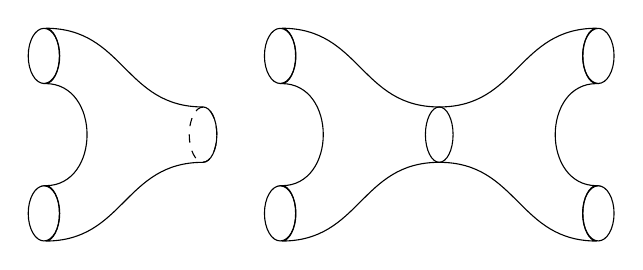
\begin{tikzpicture}[tqft/flow=east]
        \node[tqft/pair of pants, draw, rotate = 180] at (-3,0) (a) {};
        \draw (-4.02,-1) ellipse (0.2cm and 0.35cm);
        \draw (-4.02,+1) ellipse (0.2cm and 0.35cm);
        \draw[dashed] (-2,0) ellipse (0.175cm and 0.35cm);
        
        \node[tqft/pair of pants,draw,rotate=-180] (b) {};
        \draw (-1.02,-1) ellipse (0.2cm and 0.35cm);
        \draw (-1.02,+1) ellipse (0.2cm and 0.35cm);
        %\draw[dashed] (1,0) ellipse (0.175cm and 0.35cm);

        \node[tqft/pair of pants, draw] at (2,0) (b) {};
    \draw (3.02,-1) ellipse (0.2cm and 0.35cm);
        \draw (3.02,+1) ellipse (0.2cm and 0.35cm);
        %\draw[dashed] (1,0) ellipse (0.175cm and 0.35cm);
        
    \end{tikzpicture}
    \caption{The \textit{pair of pants} and a composition between two pair of pants.}
\end{figure}

\begin{rem}
In the composition, $B \coprod_{M'} B'$ we haven't said how to put a smooth structure on it. However it turns out that any choice will lead to diffeomorphic stuff. 
\end{rem}

Next we want to talk a little bit about monoidal catgories. Basically these are categories which sort of model the category of vector spaces in the sense that they have a \say{product} $\otimes$ (tensor product in vector spaces, tensor product of $R$-modules...)

A \textit{symmetric monoidal category} is a category $\ccal$ equipped with a functor $\otimes \colon \ccal \times \ccal \to \ccal$ and a unit object $\mathbf{1}_{\ccal} \in \ccal$, together with natural isomorphisms 
\begin{align*}
    C \otimes \mathbf{1}_{\ccal} & \cong  C\\
    C \otimes D & \cong D \otimes C\\
    C \otimes (D \otimes E)& \cong ( C \otimes D) \otimes E
\end{align*}
so that $\otimes$ is commutative and associative with unit $\mathbf{1}_{\ccal}$. These are subject to further coherence relations.

\begin{ej}
Let $n >0 $. The category $\textbf{Cob}(n)$ can be endowed with the structure of a symmetric monoidal category where the tensor product $\otimes \colon \textbf{Cob}(n) \times \textbf{Cob}(n) \to \text{Cob}(n)$ is given by the disjoint union of manifolds, where the unit object is the empty set (the empty set can be regarded as a manifold of any dimension; in this case, of dimension $(n-1)$). 
\end{ej}


We will be interested in a subclass of functors, namely those between monoidal categories which respect the product operation $\otimes$. We call such functors \textit{symmetric monoidal functors}. More concretely, $F \colon \ccal \to \dcal$ is a symmetric monoidal functor between two symmetric monoidal categories if it is a functor $F \colon \ccal \to \dcal$ between the underlying categories, together with natural isomorphisms 
$$F(C \otimes C') \cong F(C) \otimes F(C') \; \quad F(\mathbf{1}_{\ccal}) \cong \mathbf{1}_{\dcal} \ .$$

These isomorphisms need to be compatible with the commutativity and associativity constraints on the tensor products in $\ccal$ and $\dcal$. 


\begin{defi}[Atiyah]
Let $k$ be a field. A \textit{topological field theory} of dimension $n$ is a symmetric monoidal functor 
$$Z \colon \textbf{Cob}(n) \to \textbf{Vect}(k) \, .$$
\end{defi}


If we unravel this definition, what it means to specify a topological field theory $Z$ of dimension $n$ is the following data:
\begin{enumerate}[label = \roman*)]
    \item an vector space $Z(M)$ for every closed oriented manifold $M$ of dimension $n-1$, 
    \item a linear map of vector spaces $Z(B) \colon Z(M) \to Z(N)$ for every oriented bordism $B \colon M \to N$, 
    \item a collection of isomorphisms $Z(\emptyset) \cong k$ and 
    $$Z \left( M \coprod N\right) \cong Z(M) \otimes Z(N) \,.$$
\end{enumerate}
Again, these data has to satisfy natural coherence properties.. 

\subsection{Lower Dimensional Manifolds}
\label{lower_dimensional}

Consider a closed oriented manifold $M$ of dimension $n$. By thinking of $M$ as a bordism from the empty set (a an $(n-1)$-dimensional manifold) to itself. Hence, $M$ determines a morphism $\emptyset \to \emptyset$ in the category $\textbf{Cob}(n)$. Then, if we are given a topological field theory $Z$, then $M$ induces a map 
$$Z(M) \colon Z(\emptyset) \to Z(\emptyset) \, .$$

Since in particular, $Z$ is a tensor functor, it preserves unit objects. Hence, $Z(\emptyset)$ is the unit object in the category of vector fields over $k$, and thus it is canonically isomorphic to $k$ itself. Therefore, the induced map $Z(\emptyset)$ can be identified with an endomorphism $k \to k$, given by multiplication by some scalar $\lambda$. Identifying this endomorphism with $\lambda$ itself, we are able to extract a \say{number} off of $Z(M)$. Thus is, a topological field theory $Z$ assigns to every closed oriented manifold of dimension $n$. We wish to think of the number $\lambda$ as a \textit{diffeomorpism invariant} for closed manifold of dimension $n$. In other words, we are able to evaluate a topological field theory $Z$ of dimension $n$ not only on closed manifolds of dimension $(n-1)$, but also on manifolds with boundary and manifolds of dimension $n$.

If we cared for these diffeomorphism invariants, the study of topological field theories can be viewed as providing a set of tools to help us compute the invariants $Z(M)$ associated to closed manifolds of dimension $n$. 


Recall that a commutative Frobenius algebra $A$ over a field $k$ gives rise to a $2$-dimensional topological field theory $Z$. In particular we can evaluate $Z$ on closed oriented $2$-manifolds. These are classified, up to orientation-preserving diffeomorphism, by a single invariant $g$, the \textit{genus}.

Therefore, for each non-negative integer $g \geq 0$, we can evaluate $Z$ on a closed surface $\Sigma_g$ of genus $g$ to obtain an element $Z(\Sigma_g) \in k$. 

\begin{ej}
If $g = 0$. then $\Sigma_g$ is diffeomorphism to a 2-sphere $\mathbb{S}^2$, which we choose to view as obtained by gluing together the two hemispheres $\mathbb{S}^2_+$ and $S^2_-$ along the equator $\mathbb{S}^2_+ \cap \mathbb{S}^2_- \cong \mathbb{S}^1$. Hence, $Z(\mathbb{S}^2)$ is obtained by composing the linear maps 
$$k \cong Z(\emptyset) \xrightarrow{Z(S^2_-)} Z(\mathbb{S}^1) \xrightarrow{Z(\mathbb{S}^2_+)} Z(\emptyset) \cong k \, .$$

Now, $Z(\mathbb{S}^1)$ coincides with the Frobenius algebra $A$, $Z(\mathbb{S}_-^2) \colon k \to A$ correspond to the inclusion of the identity element of $A$ and $Z(\mathbb{S}^2_+) \colon A \to k$ is the trace map $\text{tr}$. Then it follows that the invariant $Z(\Sigma_g)$ is given by $\text{tr}(1) \in k$.
\end{ej}

\begin{ej}
If $g = 1$, then we $\Sigma_g \cong \mathbb{S}^1 \times \mathbb{S}^1$, the torus, which we can decompose as a pair of cyclinders meeting in a pair of circles. The resulting invariant $Z(\Sigma_g)$ is equal to the trace of $\ide_A$, or in other words, the dimension of the Frobenius algebra $A$. More generally, it is possible to continue with this and compute all of the invariants $\{Z(\Sigma_g)\}_{g \geq 0}$ in terms of the structure constants for the multiplication and trace on $A$.
\end{ej}

We would like to generalize the reasoning above to work in any dimension. Let $Z$ be a topological field theory of dimension $n$ and let $M$ be a closed oriented $n$-manifold, which we regard as a morphism from the empty set to $\partial M$. Then, $Z(M) \colon Z(\emptyset) \to Z(\partial M)$ can be regarded as an element of the vector space $Z(\partial M$. Now, suppose we are given a closed $(n-1)$-dimensional submanifold $N \subset M$ which partitions $M$ into two pieces $M_0$ and $M_1$. Then, $Z(M)$ is the image of 
$$Z(M_0) \otimes Z(M_1) \in Z(\partial M_0) \otimes Z(\partial M_1) \cong Z(\partial M) \otimes Z(N) \otimes Z(\overline{N})$$
under the map $Z(\partial M) \otimes Z(M) \otimes Z(\overline{N}) \to Z(\partial M)$ induced by the perfect pairing 
$$Z(N) \otimes Z(\overline{N}) \to k \, .$$

Therefore, the invariant $Z(M)$ can be computed by choosing any decomposition of $M = M_0 \amalg_N M_1$ along a closed submanifold $N$ of codimension 1. The question then is: can we do this all the time? Can we break $M$ down such that any $n$-manifold can be assembled by gluing together manifolds appearing in the list $\{M_{\alpha}\}$ along components of their boundaries? For example, it would be ideal to say, for example, triangulate $M$, and being able to compute the invariant $Z(M)$ by using the combinatorics of the triangulation

We can do it for $n = 2$, as every oriented surface $\Sigma$ can be obtained by gluing together disks, cylinders and pair of pants. However, this gets unreasonable for large $n$. Moreover, our current definition of a topological field theory does not allow any kind of flexibility in order to work with manifolds of lower dimensions instead of simply manifolds of dimension $n$ and $(n-1)$. For this reason, we introduce the following definition/remark: 

\begin{defi}
\label{extended_tft}
Let $k$ be a field. A topological field theory $Z$ gives rise to the following data:

\begin{enumerate}[label = \arabic*)]
    \item For every closed oriented $n$-manigold $M$, an element $Z(M) \in k$. 
    \item For every closed oriented $(n-1)$manifold $M$, a $k$-vector space $Z(M)$. When $M$ is empty, the vector space $Z(M)$ is canonically isomorphic to $k$.
    \item For every oriented $n$-manifold $M$, and element $Z(M)$ of the vector space $Z(\partial M)$. in the special case where $M$ is closed, this should coincide with the element specified by $1)$ under the isomorphism $Z(\partial M) = Z(\emptyset) \cong k$ of $2)$.
\end{enumerate}
A \textit{$2$-extended topological field theory} consists of the data above together with the following: 
\begin{enumerate}[resume]
    \item For every closed oriented $(n-2)$-manifold $M$, a $k$-linear category $Z(M)$ (the morphisms carry a $k$-vector space structure and composition is given by bilinear maps). Whenever $M$ is empty, $Z(M)$ should be canonically equivalent fo $\textbf{Vect}(k)$. 
    \item For every oriented $(n-1)$-manifold $M$, and object $Z(M)$ of the $k$-linear category $Z(\partial M)$. in the special case where $M$ is closed, $Z(M)$ should coincide with the vector space specified by $2)$ under the equivalence $Z(\partial M) = Z(\emptyset) \cong \vecto(k)$ of $4)$.
\end{enumerate}
\end{defi}




Notice that even though Definition \ref{extended_tft} gets us a bunch of invariants, we lose information about the linear maps $Z(B) \colon Z(M) \to Z(N)$ for a bordism $B \colon M \to N$ between oriented $(n-1)$-manifolds. We would also need to demand some coherence conditions describing $Z(B)$ whenever $B$ is obtained by gluing bordisms together, or as a disjoint union of bordisms, etcetera. 


In the case of non-extended topological field theories, the categorical data is given by a functor from the category $\textbf{Cob}(n)$ to the category $\text{Vect}(k)$. Definition \ref{extended_tft} has an analogue: strict $2$-categories. 


\begin{defi}
\label{strict_2_category}
A \textit{strict $2$-category} is a \say{category enriched over categories}. In other words, a $2$-strict category $\ccal$ consists of the following data: 
\begin{itemize}
    \item A collection of objects. 
    \item For every pair of objects $X, Y \in \ccal$, a category $\text{Map}_{\ccal}(X,Y)$. The objects of $\text{Map}_{\ccal}(X,Y)$ will be called \textit{$1$-morphisms}.The morphisms between these $1$-morphisms will be called \textit{$2$-morphisms}. The composition law of $2$-morphisms will be called \textit{vertical composition}. 
    \item For every triple of objects $X, Y, Z \in \ccal$, a \textit{composition functor}
    
    $$\text{Map}_{\ccal}(X,Y) \times \text{Map}_{\ccal}(Y,Z) \to \text{Map}_{\ccal}(Y,Z) \, .$$
    The image of a pair of 1-morphisms on the left hand side will be called the \textit{composition of $F$ and $G$}, $G \circ F$. On the other hand, the induced map on 2-morphisms will be called the \textit{horizontal composition}. 
\end{itemize}
The data above is required to satisfy the following conditions:
\begin{enumerate}[label = \arabic*)]
    \item The collection of objects together with the set of $1$-morphisms endowed with composition of $1$-morphisms is a category. 
    \item Horizontal composition of $2$-morphisms is associative. 
    \item The identity $2$-morphisms $\ide_{\ide_X}$ of the identity $1$-morphism $\ide_X$ is a unit for horizontal composition. 
\end{enumerate}
\end{defi}

\begin{ej}
\label{2_category_vect}
Given a field $k$, there is a strict 2-category $\vecto_2(k)$ whose objects are cocomplete $k$-linear categories (cocomplete here means closed under the formation of direct sums and cokernels), and given a pair of $k$-liner categories $\ccal, \dcal \in \vecto_2(k)$, $\text{Map}_{\textbf{Vect}_2(k)}(\ccal, \dcal)$ is the category of \textit{cocontinuous $k$-linear functors} from $\ccal$ to $\dcal$, that is, functors $F \colon \ccal \to \dcal$ which preserve cokernels and direct sums, and such that for every pair of objects, the induced map by $F$ is $k$-linear. 
\end{ej}

A possible idea would be to try and define a 2-extended topological field theory as a functor from an analogue version of $\textbf{Cob}(n)$ in the context of strict $2$-categories to $\vecto_2(k)$ defined in Example \ref{2_category_vect}. One could attempt to give the following:

Define, for every $n \geq 2$, a strict 2-category $\text{Cob}_2(n)$, called the \textit{extended bordism category} as:
\begin{itemize}
    \item The objects of $\text{Cob}_2(n)$ are closed oriented manifolds of dimension $(n-2)$. 
    \item Given a pair of objects $M, N \in \textbf{Cob}_2(n)$, define a category $\ccal = \text{Map}_{\textbf{Cob}_2(n)}(M,N)$ as follows:
    \begin{itemize}
        \item The objects of $\ccal$ are bordisms from $M$ to $N$.
        \item Given a pair of objects $B, B' \in \ccal$ we let $\Hom_{\ccal}(B,B')$ denote the collection of all oriented diffeomorphism classes of oriented bordisms $X$ from $B$ to $B'$, where we are further requiring $X$ to reduce to the trivial bordism along the common boundary $\partial B \cong \overline{M} \amalg N \cong \partial B'$, so that $X$ can be regarded as an $n$-manifold with boundary.
    \end{itemize}
\end{itemize}


This definition is problematic, since a strict 2-category requires \textit{strict} associativity. If $B$ is a bordism from $M$ to $M'$ and $B'$ is another bordism from $M'$ to $M''$, we would like to define a composition law $\mu(B,B')$ to be the bordism obtained by gluing $B$ to $B'$ along $M'$. This is problematic again since, first of all, we need to endow $\mu(B,B')$ with a smooth structure, which requires additional choices. On the other hand, given a triple of composable bordisms, we are required to have (strict) \textit{equality} of bordisms 
$$(B \amalg_{M'} B') \amalg_{M''} B'' = B \amalg_{M'} (B' \amalg_{M''} B'') \, ,$$
which may be difficult, since in practice there is usually a canonical homeomorphism from the left to the right hand side (which if correctly dealt with the first issue, can be promoted to a diffeomorphism). 


In order to remedy it, we will need a more relaxed version of the theory of strict 2-categories. This can be accomplished by replacing the strict $2$-category $\textbf{Cob}_2(n)$ with a non-strict 2-category, also known as \text{weak 2-categories} or \text{bicategories}, where we do not require composition to be strictly associative by only up to coherent isomorphism. Our definition of an extended topological field theory then goes as follows:

\begin{defi}
Let $k$ be a field. A \textit{2-extended topological field theory} of dimension $n$ is a symmetric monoidal functor $Z \colon \textbf{Cob}_2(n) \to \vecto_2(k)$ between 2-categories.
\end{defi}

\begin{rem}
Notice that in order to make sense of the definition above, one needs not only to think of the categories mentioned above as 2-categories, but also as symmetric monoidal 2-categories. For $\textbf{Cob}_2(n)$ this is straightforward, as the disjoint union of manifolds is a tensor product. However, in order to define tensor product on $\vecto_2(k)$, one needs to be more careful .
\end{rem}


\begin{rem}
There is a way to recover the ordinary categorical definition of a topological field theory. If $\ccal$ is an arbitrary symmetric monoidal 2-category, we can extract a symmetric monoidal category $\Omega \ccal = \text{Map}_{\ccal}(\mathbf{1}, \mathbf{1})$ of morphisms from the unit object to itself in $\ccal$. Under this construction we obtain equivalences 
$$\Omega \vecto_k(k) \cong \vecto(k) \, \; \Omega \textbf{Cob}_2(n) \cong \textbf{Cob}(n) \, .$$

Therefore, any 2-extended field theory $Z$ determines a symmetric monoidal functor $\Omega Z$ which we can think of as an $n$-dimensional topological field theory.
\end{rem}

Now, 2-extended topological field theories, even though they offer a great deal more information than its underlying topological field theory, have some issues. In order to compute $Z(M)$ for a closed oriented $n$-manifold $M$, we cut it along closed submanifolds of codimension 1, hoping that the value of $Z$ on these $(n-1)$-manifolds is somehow easier to compute. But there is no reason to think this will be the case, especially for large values of $n$. Given such a codimenion 1 closed submanifld $N$, we may attempt to iterate our construction and cut it along closed $(n-2)$-submanifolds. But then again we run into the same issues, since these new submanifolds may again be not as easy to compute as one would like them to.

This exemplifies the need for an even more extended version of topological field theories, which leads to the notion of $n$-categories. 


\begin{defi}
Let $n$ be a non-negative integer. By induction, a \textit{strict $n$-category} is defined by: 
\begin{itemize}
    \item If $n = 0$, a strict $n$-category is simply a set. 
    \item If $n >0$, a strict $n$-category is a category enriched over strict $(n-1)$-categories. In other words, a strict $n$-category $\ccal$ consists of the following data: 
    \begin{enumerate}[label = \arabic*)]
        \item A collection of objects. 
        \item For every pair of objects $X, Y \in \ccal$, a strict $(n-1)$-category $\text{Map}_{\ccal}(X,Y)$. 
        \item Identity objects $\ide_X \in \text{Map}_{\ccal}(X,X)$ for each object $X \in \ccal$, together with composition maps 
        $$\text{Ma`}_{\ccal}(X,Y) \times \text{Map}_{\ccal}(Y,Z) \to \text{Map}_{\ccal}(X,Z) \, ,$$
        satisfying the usual unit and associativity conditions. 
    \end{enumerate}
\end{itemize}
Let $\ccal$ be a strict $n$-category. For every pair of objects $X, Y \in \ccal$ we will call the collection of morphisms $f \colon X \to Y$ the \textit{$1$-morphisms} of $\ccal$. Given a pair of objects $X, Y \in \ccal$ and a pair of morphisms $f, g \colon X \to Y$, a morphism from $f$ to $g$ will be called a \textit{$2$-morphisms}. Similarly, given $2 < m \leq n$, an \textit{$m$-morphisms} is a morphism between two $(m-1)$-morphisms in $\ccal$. 

Moreover, these morphisms are equipped with various different notions of compositions, generalizing the ones given in Definition \ref{strict_2_category}, which have to be strictly associative at every level. 
\end{defi}


If $n = 1$ we recover the definition of an ordinary category. If $n = 2$, the definition above leads to a strict 2-category (Definition \ref{strict_2_category}. However, asking for strict associativity is a rather strict constraint. Instead, we would rather work with associativity up to isomorphism, which leads to the definition of a \textit{weak $n$-category} or \textit{$n$-category} for short. 



Given a pair of non-negative integers $k \leq n$, we would like to generalize the definition of the 2-extended bordism category to a $k$-category. A potential candidate would be the following: let $\text{Cob}_k(n)$ denote the $k$-category described informally as 
\begin{itemize}
    \item The objects are closed oriented $(n-k)$-manifolds.
    \item Given a pair of objects $M, N \in \textbf{Cob}_k(n)$, a 1-morphism is a bordism from $M$ to $N$.
    \item Given a pair of objects $M, N \in \textbf{Cob}_k(n)$ and a pair of bordisms from $B, B' \colon M \to N$, a 2-morphism from $B$ to $B'$ is a bordism from $B$ to $B'$, which is required to be trivial along the boundary.
    \item ...
    \item A $k$-morphism in $\textbf{Cob}_k(n)$ is an $n$-manifolds $X$ with corners, where the structure of $\partial X$ is determined by the source and target of the morphism.
    \item Composition of morphisms at all levels is given by gluing bordisms.
\end{itemize}

\begin{rem}
This is an example of a $k$-category which is not strict, as gluing of bordisms is at best associative up to diffeomorphism. 

Also, notice that if $k = 1$, then $\text{Cob}_1(n)$ is the usual bordism category $\textbf{Cob}(n)$, and if $k = 0$, one can identify $\textbf{Cob}_k(n)$ with the set of diffeomorphism classes of closed, oriented $n$-manifolds. 
\end{rem}


As we have discussed in this section, it is natural to ask for a triangulation of a closed oriented $n$-manifold $M$ in order to recover the diffeomorphism invariant $Z(M) \in k$ by means of the combinatorics of the triangulation. Hence, we will consider the case $k = n$ above, $\textbf{Cob}_n(n)$, where the objects are simply given by $0$-dimensional manifolds. Instead of working with an $n$-categorical modification of the category $\vecto(k)$, we will adopt a more general definition by working instead with any $n$-category $\ccal$. 

\begin{defi}
\label{extended_tft}
Let $\ccal$ be a symmetric monoidal $n$-category. An \textit{extended $\ccal$-valued topological ifeld theory of dimension $n$} is a symmetric monoidal functor 
$$Z \colon \textbf{Cob}_n(n) \to \ccal \, .$$
\end{defi}


Once again, this definition raises some issues. Judging only by the information required in Definition \ref{extended_tft}, we now obtain a wide range of invariants for closed manifolds of any given dimension. However, if we believe the reasoning behind that lead us to the definition above, the $n$-category $\textbf{Cob}_n(n)$ should really be encoding that an extended topological field theory $Z$ allows us compute $Z(M)$ by cutting the $n$-manifolds $M$ into more elementary pieces. If this were possible, then specifying an extended topological field theory $Z$ should not entail that much data. We have done this in the case where $n = 1$, were we have seen that a $1$-dimensional topological field theory $Z$ is determined by a single space, namely, by evaluating $Z$ on a single point. What this says is that a 1-dimensional topological field theory with values on $\ccal$ can be identified with the objects of $\ccal$. 


This is a bit too much to expect. For example, if $M$ is a closed manifold of dimension $n$, every point $x \in M$ locally looks like $\mathbb{R}^n$ for some $n$, meaning that there is a diffeomorphism of $\mathbb{R}^n$ with an open neighbourhood of $x$ in $M$. But this diffeomorphism is not unique. More precisely, we obtain a canonical diffeomorphism from an open neighbourhood of $x$ to an open ball in the tangent space $T_{M,x}$ of $M$ at $x$\footnote{This diffeomorphism is still not unique, but it is determined up to a contractible space of choices if we require its derivative at $x$ to reduce to the identity map $T_{M,x} \to T_{M,x}$.}. When $n =1$, an orientation on $M$ allows us to trivialize the tangent bundle $T_M$, so the issue of not having canonical isomorphism does not arises. However, for $n >1$, the potential non-triviality of $T_M$ is an issue. 

On the other hand, we know that for $n = 1$, it is not even true that giving a $\ccal$-valued topological field theory is equivalent to giving an object of $\ccal$, not even when $\ccal = \vecto(k)$. As we know, a $1$-dimensional topological field theory $Z$ is uniquely determined by a single vector space $V = Z(*)$, which needs to be finite dimensional. This suggest that we should impose some sort of finiteness conditions on the objects of $\ccal$.


Addressing the first issue discussed above is simpler than the second one, which we will take care of in more detail after introducing the more general notion of $(\infty, 1)$-categories. The finiteness condition we are after is called being \textit{fully dualizable}. In the case where $n = 1$ and $\ccal$ is the category of vector spaces over a field $k$, an object $V \in \vecto(k)$ is fully dualizable precisely if it is finite dimensional. 

\begin{defi}
Let $M$ be an $m$-manifold. A \textit{framing} of $M$ is a trivialization of the tangent bundle of $M$. 
\end{defi}

We introduce a variant of the $n$-category $\textbf{Cob}_n(n)$, $\textbf{Cob}^{fr}_n(n)$, where we require that all manifolds be equipped with an $n$-framing. Then, given a symmetric monoidal $n$-category $\ccal$, a \textit{framed extended topological field theory} with values in $\ccal$ is a symmetric monoidal functor 
$$Z \colon \textbf{Cob}^{fr}_n(n) \to \ccal$$
between $n$-categories. 


\begin{thm}[Baez-Dolan Cobordism Hypothesis (\cite{baez})]
\label{baez_dolan}
Let $\ccal$ be a symmetric monoidal $n$-category. Then the evaluation functor 
$$Z \mapsto Z(*)$$
determines a bijective correspondence between (isomorphisms classes of) framed extended $\ccal$-valued topological field theories and (isomorphism classes of) fully dualizable objects of $\ccal$. 
\end{thm}

\begin{rem}
A complete proof of Theorem \ref{baez_dolan} for the case when $n = 2$ can be found in \cite{chris}.
\end{rem}

\subsection{Diffeomorphism Groups}
\label{diffeomorphism_groups}

So far we have seen that a motivation towards a more general language of higher category theory comes from extended topological field theories. Here we present another example to motivate these constructions. 


Let $k$ be a field. Given a $k$-algebra $A$, one can associate to it a family of commutative algebras (where composition in $\ext$ is given by the Yoneda product)
$$HH^n(A) := \ext_{A^e}^n(A, A) \, .$$

This is known as the \textit{Hochschild cohomology of $A$}. It is particularly important, for example, if we are given an affine variety, $X = \spec A$, to which we can associate said cohomology groups by `
$$HH^k(X) := HH^k(A) \, .$$

Moreover, we can generalize this construction to more complicated spaces, by picking an affine cover of $X$, taking Hochschild cohomology of these affine pieces and gluing them in an appropriate manner. 

Let $X$ be a smooth variety of dimension $n$ over $\mathbb{C}$. Then (with a minor argument on the dimension of $X$), a version of the Hochschild-Kotant-Rosenberg Theorem tell us that to compute the $2n$-th Hochschild cohomology is equivalent to taking the $n$-th cohomology of $X$ with coefficients on the top-wedge power of its tangent bundle. In other words, 
$$HH^{2n}(X) \cong H^n(X, \wedge^n \tcal_X) \, .$$

If we had the cotangent bundle instead of the tangent bundle, then Serre duality says that there is a canonical trace map 
$$H^n(X, \wedge^n \tcal^*_X) \to \mathbb{C}$$
which will endow $HH^{2n}(X)$ with the structure of a \say{commutative} Frobenius algebra, and hence it gives rise to a $2$-dimensional topological quantum field theory using the folk Theorem stated earlier. If $X$ is Calabi-Yau, then the top-wedge power of its tangent bundle is trivial, and so is the top-wedge power of its cotangent bundle. Therefore, if $X$ is Calabi-Yau, we get a canonical trace map as discussed above.

\begin{rem}
The product in Hochschild cohomology is commutative in the graded sense, not in the usual one, although this detail is not really important. 
\end{rem}



This phenomenon is common among examples of topological field theories $Z$; that is, sometimes the vector spaces $Z(M)$ are naturally given some kind of homology or cohomology, as it was the case for $2$-dimensional topological field theories where we have seen that evaluating $Z$ on a circle is given by computing the Hochschild cohomology of some space. We could try to make this more precise by introducing a modification on the definition of topological field theories. These were seen as functors which send $(n-1)$-manifolds to vector spaces. Now, we wish to promote such functors to functors that take values on the category of chain complexes. 

In practice, we would start with an $n$-dimensional topological field theory 
$$Z \colon \textbf{Cob}(n) \to \vecto(k)$$
which we would like to promote to a symmetric monoidal functor 
$$\overline{Z} \colon \textbf{Cob}(n) \to \textbf{Ch}(k) \, .$$

In particular, this means that for every closed oriented manifold $M$ of dimension $(n-1)$ we should obtain a chain complex whose homology coincides with the value $Z(M)$, and that for every oriented bordisms $B \colon M \to N$ between $(n-1)$-manifolds, a chain map 
$$\overline{Z}(B) \colon \overline{Z}(M) \to \overline{Z}(N)$$
obtained from $Z(B) \colon Z(M) \to Z(N)$ by passing to homology. 

Now, suppose we are given a pair of bordsisms $B, B' \colon M \to N$ together with an orientation-preserving diffeomorphism $\phi \colon B \to B'$ which is the identity on $\partial B$. One would expect that $\overline{Z}(B) = \overline{Z}(B')$ as chain map. However, this is too strong of an assumption to make, since for example, the chain map $\overline{Z}(B)$ may require some further choice of additional data on $B$, which might not be diffeomorphism invariant. 

However, since we know that $Z(B) = Z(B')$ in the usual topological field theory sense, a more reasonable assumption to make is that of the exitence of a chain homotopy between $\overline{Z}(B)$ and $\overline{Z}(B')$, since in the end, it will agree with our expectations by passing to homology. However, this comes with a cost, as this chain homotopy depends on a choice of a diffeomorphism $\phi \colon B \to B'$, which requires to keep track of diffeomorphism groups of bordisms. 




The discussion above suggests that an $n$-dimensional topological field theory should be, roughly speaking, an assignment of the form 
\begin{align*}
    \text{closed $(n-1)$-manifolds} & \longrightarrow \text{chain complexes}\\
    \text{bordisms} & \longrightarrow \text{chain maps}\\
    \text{diffeomorphisms between bordisms} & \longrightarrow \text{chain homotopies}\\
\end{align*}

However there is no reason to stop there, since again, we have a notion of \say{sameness} in the context of diffeomorphisms, i.e. isotopies. It makes sense to continue by further expanding the assignment to allow for
\begin{align*}
    \text{isotopies} & \longrightarrow \text{chain homotopies between chain homotopies}\\
    \cdots & \longrightarrow \cdots
\end{align*}

This sort of construction arises more naturally in the context of higher category theory. More precisely, an $n$-dimensual chain-valued topological field theory should be seen as a functor 
$$Z \colon \textbf{Cob}_t(n) \to \textbf{Ch}_t(k)$$
between $(\infty, 1)$-categories (that is, where all $k$-morphisms are invertible for $k>1$), where 
\begin{itemize}
    \item The objects of $\textbf{Cob}_t(n)$ are closed, oriented $(n-1)$-manifolds.
    \item The 1-morphisms are oriented bordisms.
    \item The 2-morphisms are orientation-preserving diffeomorphisms.
    \item The 2-morphisms are isotopies between (orientation-preserving) diffeomorphisms.
    \item So on and so forth. 
\end{itemize}
and $\textbf{Ch}_t(k)$ as as objects chain complexes, 1-morphisms chain maps, 2-morphisms chain homotopies,...


To summarize the various bordisms categories we have introduced so far (the $n$-category $\textbf{Cob}_n(n)$, the ordinary bordism category $\textbf{Cob}(n)$ and now $\textbf{Cob}_t(n)$), we notice that:
\begin{itemize}
    \item Objects of $\textbf{Cob}(n)$ and $\textbf{Cob}_t(n)$ are the same, and morphisms in $\textbf{Cob}(n)$ are isomorphism classes of 1-morphisms in $\textbf{Cob}_t(n)$. In other words, $\text{Cob}_t(n)$ can be regarded as an improvement from $\textbf{Cob}(n)$ by allowing higher morphisms, which keep track of the diffeomorphism groups of $n$-manifolds (instead of identifying diffeomorphic $n$-manifolds).
    \item Objects and morphisms of $\textbf{Cob}(n)$ can be regarded as $(n-1)$ morphisms and $n$-morphisms of $\textbf{Cob}_n(n)$, so we can think of $\textbf{Cob}_n(n)$ as an improvement from $\textbf{Cob}(n)$ obtained by considering lower morphisms which correspond to manifolds of dimension lower than $(n-1)$. 
\end{itemize}

If we were interested only in one of the advantages displayed so far, we could consider these definitions separately. However, we can combine these definitions using the language of $(\infty, n)$-categories (where all $k$-morphisms for $k>n$ are now assumed to be invertible) and treat both points of view simultaneously. For now, we sketch the following definition: 

\begin{defi}
\label{infinity_n_bordism}
Let $n$ be a non-negative integer. The $(\infty, n)$-category $\textbf{Bord}_n$ is (informally) described as follows:
\begin{itemize}
    \item The objects of $\textbf{Bord}_n$ are 0-manifolds. 
    \item The 1-morphisms of $\textbf{Bord}_n$ are bordisms between 0-manifolds. 
    \item The 2-morphisms of $\textbf{Bord}_n$ are bordisms between bordisms between 0-manifolds. 
    \item ...
    \item The $n$-morphisms of $\textbf{Bord}_n$ are bordisms between bordisms between... between bordisms between 0-manifolds (this correspond with $n$-manifolds with corners). 
    \item The $(n+1)$-morphisms of $\textbf{Bord}_n$ are diffeomorphisms which reduce to the identity on the boundaries.
    \item The $(n+2)$-morphisms of $\textbf{Bord}_n$ are isotopies of diffeomorphisms.
    \item ...
\end{itemize}
\end{defi}

Furthermore, as it was the case in the previous versions of the bordism category, the $(\infty, n)$-category $\textbf{Bord}_n$ is equipped with a symmetric monoidal structure given by disjoint unions of manifold. In a similar fashion as described in \ref{lower_dimensional}, we can circumvent the difficulties arising from the potential non-trivalization of the tangent bundle $T_M$, by adapting Definition \ref{infinity_n_bordism} to obtain the framed bordism $(\infty, n)$-category $\textbf{Bord}_n^{fr}$. 

Theorem \ref{baez_dolan} admits an $(\infty, n)$-categorical analogue, which we state here. 



\begin{thm}[Cobordism Hypothesis]
\label{cobordism_hypothesis}
Let $\ccal$ be a symmetric monoidal $(\infty, n)$-category. The evaluation functor $Z \mapsto Z(*)$ determines a bijection between isomorphism classes of symmetric monoidal functors $\textbf{Bord}_n^{fr} \to \ccal$ and isomorphism classes of fully dualizable objects of $\ccal$. 
\end{thm}



\section{Higher Category Theory}
\label{section_2}
 
We have seen already the need of a notion of an $n$-category. Inductively, an $n$-category $\ccal$ should consist of a set of objects $X, Y, Z, \dots$ together with an $(n-1)$-category $\text{Map}_{\ccal}(X,Y)$ for every pair of objects, equipped with associative and unital composition law. In the case we are mostly interested, namely, the theory of bordisms developed in the previous talks, this almost fit this pattern. However, the commutativity conditions of our diagrams are met only up to isomorphism. Hence it seems natural to replace the commutativity requirement by a more relaxed notion. This comes with a price, however, that in order to specify these structures one needs an insane amount of conditions, which are feasible for some small values of $n$, but impossible for higher $n$.

Instead, we will adopt a different approach. Theorem \ref{cobordism_hypothesis} is naturally stated in the language of $(\infty, n)$-categories, which were informally defined by having a collection of objects, together with higher morphisms with the contraint that for $k >n$, all $k$-morphisms of an $(\infty, n)$-category are required to be invertible. Inductively, we would like to think of $(\infty, n)$-categories as \say{enriched} over $(\infty, n-1)$-categories. That is, for $n >0$, an $(\infty, n)$-category $\ccal$ should consist of the following data: 

\begin{itemize}
    \item A collection of objects $X, Y ,Z, \dots$
    \item For every pair of objects $X, Y \in \ccal$, and $(\infty, n-1)$-category of $1$-morphisms, together with a composition law for $1$-morphisms which is associative and unital up to (coherent) isomorphism. 
\end{itemize}

In order to make sense of what an $(\infty, n)$-category should be, we will first consider the case where $n = 0$, leading to the notion of an $(\infty, 0)$-category, i.e. where all $k$-morphisms are invertible. This (yet to be defined) mathematical object has a name of its own, an \textit{$\infty$-groupoid}. Using the theory of homotopy types of topological spaces, we will see that the theory of $\infty$-groupoids (up to equivalence) actually corresponds to the theory of topological spaces (up to homotopy type). We will take that as our definition of $\infty$-groupoids, which will then serve as \say{building blocks} for $(\infty, 1)$-categories. 


There are different models one can adopt to define the notion of an $\infty$-groupoid, an $(\infty, 1)$-category and so on. We will sketch, for example, a more precise definition of the fundamental $\infty$-groupoid of a topological space using the theory of \textit{Kan complexes}, and briefly explain how one can \say{jump} from one definition to the other without loosing important information about the objects we are interested in. For $(\infty, 1)$-categories, a good model for intuition is that of \textit{topological categories}, where the hom-spaces are equipped with a topology. In other words, a topological category is a category $\ccal$ enriched over the category of compactly generated Hausdorff spaces\footnote{Recall that a topological space $X$ is \textit{compactly generated} if a subspace $A$ is closed in $X$ if and only if $A \cap K$ is closed in $K$ for all compact subspaces $K \subset X$. This condition is probably better viewed by solving the issue of the category of topological spaces to be cartesian closed, or by allowing the product of CW-complexes to be a CW-complex.}. In fact, one may view the $(\infty, 1)$-category $\textbf{Cob}_t(n)$ we described in \ref{diffeomorphism_groups} as a topological category. This approach is technically more difficult, so we instead define a different model for $(\infty, 1)$-categories: complete Segal spaces. Finally, seeing a complete Segal space as a simplicial space, one can iterate this construction by allowing simplicial spaces to \say{point in $n$-dimensions}. This leads to the notion of an $n$-fold complete Segal space, which we will adopt for a definition of an $(\infty, n)$-category. 


\subsection{$\infty$-groupoids}

Consider a topological space $X$. We can extract a category $\pi_{\leq 1} X$ from $X$ called the \textit{fundamental groupoid}. This category is defined as follows:
\begin{itemize}
    \item The objects of $\pi_{\leq 1} X$ are the points of $X$,
    \item A morphism from $x$ to $y$ is a homotopy class of paths in $X$ starting at $x$ and ending at $y$.
\end{itemize}

From the fundamental groupoid $\pi_{\leq 1} X$, one can recover $\pi_0(X)$, the set of path components of $X$, as the isomorphism classes of objects in the fundamental groupoid. Moreover, $\pi_1(X,x)$ of $X$ is the automorphism group of the object $x$ in $\pi_{\leq 1}(X)$.  

However, if we want to specify further information about the homotopy type of $X$ such as the higher homotopy groups $\pi_n(X,n)$ for $n \geq 2$, the fundamental groupoid of $X$ is simply not enough. We can hope to iterate this construction, and so it seems natural to define $\pi_{\leq n}(X)$, an $n$-category called the \textit{fundamental $n$-groupoid of $X$} as follows: 
\begin{itemize}
    \item The objects of $\pi_{\leq n} X$ are the points of $X$,
    \item A 1-morphism in $\pi_{\leq n} X$ from $x$ to $y$ is a path in $X$ from $x$ to $y$, 
    \item Given a pair of objects $x, y \in X$ and $1$-morphisms $f, g \colon x \to y$, a $2$-morphism from $f$ to $g$ in $\pi_{\leq n} X$ is a homotopy of paths in $X$,
    \item $\dots$
    \item An $n$-morphism in $\pi_{\leq n}X$ is given by a homotopy between homotopies between... between paths between points in $X$.
\end{itemize}

We say $\pi_{\leq n} X$ is an \textit{$n$-groupoid} because all of its $k$-morphisms are invertible for $1 \leq k \leq n$. For example, a path $p \colon [0,1] \to X$ (a $1$-morphism in $\pi_{\leq n} X$) has an inverse given by $t \mapsto p(1-t)$. 

The theory of topological spaces is \say{equivalent} to the theory of $n$-groupoids:
\begin{itemize}
    \item Let $\ccal$ be an $n$-groupoid (that is just a category in which every $k$-morphism is assumed to be invertible for $0 < k \leq n$). Then $\ccal$ is equivalent to $\pi_{\leq n} X$ for some topological space $X$. 
\end{itemize}

However, we need to be careful, since we can obtain topological spaces with equivalent fundamental groupoids. In order to capture this ambuguity, we must recall that definition of $n$-type. 

\begin{defi}
A topological space $X$ is called an \textit{$n$-type} if the homotopy groups $\pi_k(X,x)$ vanish for all $x \in X$ and all $k>n$. 
\end{defi}

With this refinement, we can correspond to any topological space $X$ and $n$-type $Y$ together with a map $f \colon X \to Y$ inducing an isomorphism on homotopy groups in degrees $\leq n$. Moreover, $Y$ is uniquely determined up to weak homotopy equivalence, and the corresponding map on the fundamental $n$-groupoids $\pi_{\leq n} X \to \pi_{\leq n} Y$ is an equivalence of $n$-catogories. We can thus refine our equivalence between theories as follows:
\begin{itemize}
    \item The construction $X \mapsto \pi_{\leq n} X$ establishes a bijective correspondence between $n$-types (up to weak homotopy equivalence) and $n$-groupoids (up to equivalence).
\end{itemize}


Now, we have separated a little bit from our goal. We want a theory of $n$-categories, and we have yet failed to accommodate a description of what such a theory should entail. $n$-groupoids should be seen as a toy example of $n$-categories, but there are various levels of complexity depending on how many of our higher morphisms are invertible. 



There is no reason to stop at level $n$. It may be convenient to allow the case $n = \infty$, in our sketch of $\pi_{\leq n} X$. If we allow this limit case, then there is no need to talk about $n$-types in our previous thesis, and hence we obtain the following: 

\begin{itemize}
    \item The construction $X \mapsto \pi_{\leq \infty} X$ establishes a bijection between topological spaces (up to weak homotopy equivalence) and $(\infty, 0)$-categories. 
\end{itemize}

We can then approach the definition of an $\infty$-groupoid as follows: 

\begin{defi}
An $\infty$-groupoid is a topological space. 
\end{defi}

Throughout the rest of the notes, we will use the notion of a topological space and $\infty$-groupoid interchangebly. 



\subsection{Kan Complexes}
\label{kan_complexes}
Of course, we have not really said anything about what the assignment $X \mapsto \pi_{\leq \infty} X$ actually assigns to a topological space $X$. Although this formalism is not really important for the development of the following sections, we introduce a different foundation. 

Let $n$ be a non-negative integer. We denote by $[n]$ the partially ordered set $\{0 < 1 < \cdots < n+1\}$. These partially ordered sets assemble into the objects of a category $\Delta$, called the \textit{simplex category}. Its objects are of the form $[n]$ for non-negative integers $n$, and a morphism $f \colon [n] \to [m]$ is a non-decreasing map, i.e. $f(i) < f(j)$ for $i<j$. A \textit{simplicial set} $K$ is a functor
$$K \colon \Delta^n \to \sets \, .$$

The definition of a simplicial set originates from algebra topology. The \textit{standard topological $n$-simplex}, denoted by $|\Delta^n|$, is the subspace of $\mathbb{R}^{n+1}$ defined as 
$$|\Delta^n| := \{(x_0, \dots , x_n) \in \mathbb{R}^{n+1} \mid x_i \geq 0 \, , \; x_0 + \cdots + x_n = 1\} \, .$$

Given a topological space $X$, we obtain a simplicial set $\text{Sing}\, X$ via the assignment 
$$[n] \mapsto \Hom_{\topo}(|\Delta^n|, X) \, .$$

What is interesting about this construction is that $\text{Sing}\, X$ remembers the relevant homotopy information of the topological space $X$. More precisely, $X$ is determined by $\text{Sing}\, X$ up to weak equivalence. Moreover, by abstract nonsense, one shows that the functor $X \mapsto \text{Sing}\, X$ admits a left adjoint: given a simplicial set $K$, we obtain a topological space $|K|$ known as the \textit{geometric realization of $K$}. For example, one gets a canonical simplicial set $\Delta^n$ by 
$$[m] \mapsto \Hom_{\Delta}([m], [n]) \, .$$
The geometric realization of this simplicial set is, unsurprisingly, $|\Delta^n|$, the standard topological $n$-simplex, defined above. 

Consider $|\Delta^n|$. The $i$-th horn of $|\Delta^n|$, denoted by $|\Lambda_i^n|$, obtained by deleting the face of $\Delta^n|$ opposite to the vertex $i$, is a retract of the standard $n$-simplex. This property is captured in a more refined setting as follows: any continuous map of topological spaces $|\Lambda_i^n| \to X$ lifts to a map $\Delta^n| \to X$, rendering the diagram 
\begin{equation*}
    \begin{tikzcd}[row sep = large, column sep = large]
    \left| \Lambda_i^n\right| \arrow[d, hook] \arrow[r] & X \\
    \left|\Delta^n\right| \arrow[ru, dotted] & 
    \end{tikzcd}
\end{equation*}
commutative for all $0 \leq i \leq n$. 

If we believe that the geometric realization of a simplicial set if left adjoint to the singular complex functor $\text{Sing}(-)$, we obtain an analogous statement by replacing the topological space $X$ in the diagram above by its singular complex $\text{Sing}\, X$. In other words, given an arrow $\Lambda_i^n \to \text{Sing}\, X$ (here $\Lambda_i^n$ denotes the $i$-th horn of $\Delta^n$, obtained by deleting the interior and the face opposite to the $i$-th vertex of $\Delta^n$), there exists an arrow $\Delta^n \to \text{Sing}\, X$ such that the diagram
\begin{equation*}
    \begin{tikzcd}[row sep = large, column sep = large]
    \Lambda_i^n \arrow[d, hook] \arrow[r] & \text{Sing}\, X \\
    \Delta^n \arrow[ru, dotted] & 
    \end{tikzcd}
\end{equation*}

This property of $\text{Sing}\, X$ deserves a name of its own, and is known as the \text{Kan complex}. More precisely:

\begin{defi}
Given a simplicial set $K$, we say that $K$ is a \textit{Kan complex} if for any $0 \le i \leq n$, any map $\Lambda_i^n \to K$ factors as 
\begin{equation*}
    \begin{tikzcd}[row sep = large, column sep = large]
    \Lambda_i^n \arrow[d, hook] \arrow[r] & K\\
    \Delta^n \arrow[ru, dotted] & 
    \end{tikzcd}
\end{equation*}
\end{defi}


The theory of Kan complexes is a \say{good model} of the theory of $\infty$-groupoids. Before, we have made a very informal argument that assigns to a topological space $X$ its $\infty$-groupoid $\pi_{\leq \infty} X$. Equipped with the notion of a Kan complex we can make this assignment more precise. 

\begin{defi}
Let $X$ be a topological space. The \textit{fundamental $\infty$-groupoid} of $X$, $\pi_{\leq \infty} X$, is defined as the singular complex of $X$. In other words, 
$$\pi_{\leq \infty} X := \text{Sing}\, X \, .$$
\end{defi}


Let us try to understand why this definition makes sense. Informally, an $\infty$-groupoid was described as a category $\ccal$ in which we allowed higher morphisms of any degree, all of which are required to be invertible. Given a category $\ccal$, we can associate to it a simplicial set $N(\ccal)$, called the \textit{nerve of $\ccal$}, whose $n$-simplices are given by functors $[n] \to \ccal$ (here $[n]$ is seen as a category where the the morphisms are given by the poset structure of $[n]$). In other words, 
$$N(\ccal)_n: = \text{Fun}_{\textbf{Cat}}([n], \ccal) \, .$$
Unravelling the definition, this means that $N(\ccal)_n$ consists of the set of all composable sequence of morphisms 
$$C_0 \to C_1 \to \cdots \to C_n$$
of length $n$, where $C_i$ are ojects in $\ccal$. 

Notice that we can recover the category $\ccal$ by the simplicial structure of its nerve. In particular, the objects of $\ccal$ are simply the $0$-simplices of $N(\ccal)$. Similarly, the set morphisms of $\ccal$ are given by $N(\ccal)_1$. The identity morphism $\ide_C \colon C \to C$ is simply the degenerate simplex $s_0(C)$. Given a pair of arrows in $\ccal$, $C_0 \xrightarrow{f} C_1 \xrightarrow{g} C_2$, we can interpret it as an arrow $\Lambda_1^1 \to N(\ccal)$. The composition law for $\ccal$ means that we can lift it to an arrow $\Delta^2 \to N(\ccal)$. We can characterize the simplicial sets which arise as the nerve of a category by making use of that observation. 

\begin{prop}[\cite{topos} Prop. 1.1.2.2]
Let $K$ be a simplicial set. The following are equivalent: 
\begin{enumerate}[label = \arabic*)]
    \item There exists a (small) category $\ccal$ and an isomorphism $K \cong N(\ccal)$. 
    \item For each $0<i<n$ and each diagram 
    \begin{equation*}
        \begin{tikzcd}[row sep = large, column sep = large]
        \Lambda_i^n \arrow[r] \arrow[d, hook] & K \\
        \Delta^n \arrow[ru, dotted] &
        \end{tikzcd}
    \end{equation*}
    there exists a \text{unique} dotted arrow rendering the diagram commutative. 
\end{enumerate}
\end{prop}

The Proposition above looks a lot like the definition of a Kan complex, with two differences: the existence of a dotted arrow $\Delta^n \to K$ is not unique whenever $K$ is a Kan complex, and the lifting condition for Kan complexes needs to be satisfied for the \textit{outer horns} $\Lambda_0^n$ and $\Lambda_n^n$. 

Suppose $K$ is a simplicial set which is the nerve of a category $\ccal$. When $i = n= 2$, the requirement of lifting an arrow $\Lambda_2^2 \to K$ to a $2$-simplex $\Delta^2 \to K$ amounts to supplying the dotted arrow 
\begin{equation*}
    \begin{tikzcd}[row sep = large, column sep = large]
    & C_2 \arrow[rd]& \\
    C_0 \arrow[ru] \arrow[rr, dotted] & & C_1
    \end{tikzcd}
\end{equation*}
which renders the diagram commutative. Similarly, an arrow $\Lambda_0^2 \to K$ is given by the diagram of solid arrows
\begin{equation*}
    \begin{tikzcd}[row sep = large, column sep = large]
    & C_1 \arrow[rd, dotted] & \\
    C_0 \arrow[rr] \arrow[ru] & & C_2
    \end{tikzcd}
\end{equation*}
Then, $K$ being a Kan complex amounts to specifying the dotted arrow in the diagram above, rendering it commutative. We can interpret these dotted arrows as providing inverses for morphisms in $\ccal$. In fact, one can show that the simplicial set $N(\ccal)$ is a Kan complex if and only if $\ccal$ is a groupoid. 





Finally, although the existence of an adjunction 

$$|-| \colon \sets_{\Delta} \longleftrightarrow \topo \colon \text{Sing}(-)$$
provides us with an identification between simplicial sets and CW-complexes (the geometric realization functor, which we have not really defined, takes values on CW-complexes). However, there is much more information on the category of CW-complexes that is not really captured by the categorical notion of an adjunction. For example,  

We can define a \say{homotopy factorization system} in $\topo$, where weak equivalences act as some sort of quasi-isomorphism, where Serre fibrations play the role of \say{nice surjections}. Then the adjunction above extends to this more general version of $\topo$ with these two classes of distinguished morphisms, so that passing from a topological space $X$ to its singular complex means that no homotopy invariant information is loss in the process. 

This (hopefully) provides some intuition as to why we would regard Kan complexes as a model of $\infty$-groupoids. 

\subsection{Topological Categories}
\label{topological_categories}

In the previous section we have introduced the notion of an $\infty$-groupoid, and argued that such mathematical object is equivalent in some sense to the more familiar notion of a topological space. In light of the informal discussion at the beginning of the section, we wish to see an $(\infty, n)$-category as \textit{enriched over $(\infty, n-1)$-categories}. Taking $n =1$, this means that the data associated to an $(\infty, 1)$-category should consist of a collection of objects together with an $\infty$-groupoid $\text{Map}_{\ccal}(X,Y)$ for every pair of objects $X, Y \in \ccal$. As we have seen, we can correspond a topological space to an $\infty$-groupoid, and this leads us to think of an $(\infty, 1)$-category as a \textit{topological category}. 

\begin{defi}
A \textit{topological category} is a category enriched over the category of compactly generated Hausdorff topological spaces.
\end{defi}

\begin{rem}
The reason why we choose to work over the category of compactly generated topological spaces rather than the usual category $\topo$ is the following. If one works with topological spaces without any further assumption, we do not get a \textit{cartesian closed structure} on the category of CW-complexes, which, as discussed before, model $\infty$-groupoids via the fundamental $\infty$-groupoid we sketched in \ref{kan_complexes}. However, for the purpose of this section, the extra requirement on our topological spaces can be ignored.
\end{rem}

 



\section{Complete Segal Spaces}
\label{complete_sega_spaces}
In the preceding sections, we have given two examples to motivate the need for a more suitable notion of a bordism category, and argued that higher category theory is the way to go: topological field theories which allow cutting by lower dimensional manifolds, and chain-valued topological field theories, which contain information about the diffeomorphism groups of bordisms. Loosely, we introduced the notion of an $(\infty, 1)$-category, and argued that for us to consider these two examples simultaneously, one needs a more solid notion of an $(\infty, n)$-category.

In this section, we set the task to construct this new toolkit in order to formulate the Cobordism Hypothesis, which is our end goal and will be treated in the next part of this notes. We have seen an approach to $(\infty, 1)$-categories using the theory of topological categories, and noted its difficulty in order to give precise definitions. Here we introduce the theory of complete Segal spaces, which allows for a more natural model of $(\infty, 1)$-categories, which we need in order to produce a good theory of $(\infty, n)$-categories. 


Assume we already have a good theory of $(\infty, 1)$-categories. We know from previous sections that the theory of $\infty$-groupoids is easy to understand in the sense that it is equivalent to the homotopy theory of topological spaces. We are now asking ourselves what happens if we plug in an $(\infty, 1)$-category. What do we get as an output? 

\begin{align*}
\left\{ \infty \text{-categories}\right\} & \longleftrightarrow \left\{ \text{topological spaces}\right\}\\
\left\{ (\infty, 1)\text{categories}\right\} & \longleftrightarrow \left\{ ???\right\} 
\end{align*}

\subsection{Segal Spaces}

The main difference of working with $(\infty, 1)$-category rather than $\infty$-groupoid is that an $(\infty, 1)$-category $\ccal$ may contain non-invertible 1-morphisms. However, we can extract an $\infty$-groupoid $\ccal_0$ from $\ccal$ as follows:
\begin{itemize}
    \item The objects of $\ccal_0$ are the objects of $\ccal$, 
    \item The 1-morphisms of $\ccal_0$ are the invertible 1-morphisms of $\ccal$, 
    \item the 2-morphisms of $\ccal_0$ are the 2-morphisms between invertible 1-morphisms of $\ccal$, 
    \item ...
\end{itemize}
Since $\ccal_0$ is an $\infty$-groupoid, we can identify it with a topological space $X_0$, namely the topological space for which $\ccal_0 \cong \pi_{\leq \infty} X_0$ . If $\ccal$ was already an $\infty$-groupoid, then $X_0$ contains all the information we could possibly care about $\ccal$. However, $\ccal_0$ forgets everything about the non-invertible 1-morphisms in $\ccal$. In order to remember this part of the structure of an $(\infty, 1)$-category, we proceed by extracting a series of $(\infty, 1)$-morphisms by inductively discarding non-invertible $k$-morphisms. We do it as follows. 

We can think of a morphism in $\ccal$ as a functor $[1] \to \ccal$, where $[1]$ denotes the ordinary category associated to the linearly ordered set $\{0<1\}$. The collection of all such functors is naturally organized into another $(\infty, 1)$-category $\text{Fun}([1], \ccal)$, where our objects are now the $1$-morphismms which we have identified as functors $[1] \to \ccal$ and the $1$-morphisms are given by natural transformation between such functors. Repeating the process of discarding non-invertible natural transformations, we can extract an $\infty$-groupoid $\ccal_1$ out of $\text{Fun}([1], \ccal)$ whih again corresponds to a topological space $X_1$ for 1-morphisms in $\ccal$. 

This topological space remembers a little bit more about our original $(\infty, 1)$-category $\ccal$. However we have lost all the information about compositions between non-invertible 1-morphisms in $\ccal$. To correct this, we can consider pairs of composable 1-morphisms 
$$X \xrightarrow{f} Y \xrightarrow{g} Z$$
in $\ccal$, which we regard as functors $[2] \to \ccal$. More generally, for every non-negative $n$, the linearly ordered set $[n] = \{0 < 1 < \cdots < n \}$ can be though of as a category (Section \ref{kan_complexes}), and the collection of all functors $[n] \to \ccal$ is naturally organized into an $(\infty, 1)$-category $\text{Fun}([n], \ccal)$, from which we can extract an $\infty$-groupoid $\ccal_n$ which we can identify with the fundamental $\infty$-groupoid of a topological space $X_n$. 


\begin{rem}
\label{teaser}
On Section \ref{topological_categories}, we saw that a natural way of visualizing $(\infty, 1)$-categories can be done in terms of topological categories. Although this framework is not really suitable for practical purposes, it is good for intuition. What I mean by that is that according to the principle that an $(\infty, 1)$-category corresponds to a topological category $\ccal$, we wish to think of the topological spaces $X_0$ and $X_1$ as classifying spaces for objects and 1-morphisms of $\ccal$, respectively. 

Notice that by construction, the (unique) map $[1] \to [0]$ obtained by \say{hitting $0$ twice} induces a map by passing through 
$$\text{Fun}([0], \ccal) \to \text{Fun}([1], \ccal)$$
which again should induce a map $\delta \colon X_0 \to X_1$. Then, if we think of $X_0$ as a classifying space for objects in the $(\infty, 1)$-category $\ccal$, this condition essentially means that every invertible $1$-morphism of $X_1$ already came from a unique path in $X_0$. In particular, a natural condition to ask for on the data of the topological spaces $\{X_n\}_{n \geq 0}$ is that the \textit{degeneracy} $\delta$ is in some sense invertible for the subspace of $X_1$ consisting of invertible $1$-morphisms. We will talk more about this when dealing with \textit{complete Segal spaces}.
\end{rem}

To summarize the construction above, we have extracted a collection of topological spaces $\{X_n\}_{n \geq 0}$ from our (yet) naive notion of an $(\infty, 1)$-category. Next, we study some question regarding the nature of these data. 

\begin{itemize}
    \item What mathematical object is $\{X_n\}_{n \geq 0}$?
    \item What features does this object possess?
    \item How much of the $(\infty, 1)$-category $\ccal$ can be recovered from the sequence $\{X_n\}_{n \geq 0}$?
\end{itemize}

As we will see: 

\begin{itemize}
    \item The topological spaces $\{X_n\}_{n \geq 0}$ are organized into a simplicial space (simplicial object in the category of topological spaces),
    \item The simplicial space associated to an $(\infty, 1)$-category is always a complete Segal space,
    \item An $(\infty, 1)$-category $\ccal$ is determined up to equivalence by the complete Segal space $\{X_n\}_{n \geq 0}$. Moreover every complete Segal space arises from an $(\infty, 1)$-category in this way. 
\end{itemize}


Let us address the first question. Given a simplicial set $K \colon \Delta^{op} \to \sets$, there are many interesting variations of the definitions depending on what our target category is. Consider for example a commutative ring $k$ together with a $k$-algebra $A$. The assignment 
$$[n] \mapsto A^{\otimes n+1}$$
determines an $k$-module for each linearly ordered set $[n]$, by defining the simplicial identities to be:
$$\partial_i(m \otimes a_1 \otimes \cdots \otimes a_n) := \begin{cases}
a_0 a_1 \otimes a_2 \otimes \cdots \otimes a_n & \text{if $i = 0$}\\
a_0 \otimes a_1 \otimes \cdots \otimes a_i a_{i+1} \otimes \cdots \otimes a_n & \text{if $0 < i < n$}\\
a_n a_0 \otimes a_1 \otimes \cdots \otimes a_{n-1} & \text{if $i = n$}
\end{cases}$$
and 
$$\sigma_i(a_0 \otimes a_1 \otimes \cdots \otimes a_n) = a_0 \otimes \cdots \otimes a_i \otimes 1 \otimes a_{i+1} \otimes \cdots \otimes a_n$$
where $m \in M$ and $a_i \in A$. In other words, the assignment $[n] \mapsto A^{\otimes n+1}$ determined a \textit{simplicial $k$-module} (i.e. a simplicial set where the $n$-simplices are equipped with a $k$-module structure). Passing to the unnormalized chain complex via the Dold-Kan correspondence, we obtain a chain complex $C(A)$, whose homology determines the \textit{Hochschild homology} of the $k$-algebra $A$, denoted by $HH_{\bullet}(A)$. 

\begin{rem}
Notice that equivalently, $C(A)$ could have been defined as $A \otimes{A^e} C^{bar}(A)$, where $C^{bar}(A)$ denotes the bar complex, which is a resolution of $A$ as an $A$-bimodule. This carries a natural cyclic action of the group $\mathbb{Z}/(n+1)$, which we will talk about later. 
\end{rem}


We can characterize the structure arising from the data $\{X_n\}_{\geq 0}$ as follows. Consider a monotone map $f \colon [m] \to [n]$. By pre-composition, this induces a map 
$$f^* \colon \text{Fun}([n], \ccal) \to \text{Fun}([m], \ccal) \, $$
which in turn induces a map 
$$f^* \colon X_n \to X_m$$
obtained by discarding the non-invertible natural transformations. 

\begin{defi}
A \textit{simplicial space} if a functor $X \colon \Delta^{op} \to \topo$.
\end{defi}

Therefore, we see that the data $\{X_n\}_{n \geq 0}$ can be succinctly described as a simplicial space.  

\begin{rem}
\label{not_inverse}
The construction introduced in the beginning of the section that takes an $(\infty, 1)$-category $\ccal$ and assigns a simplicial space $X_{\bullet}$ behaves much like the nerve of a category. In both cases, the $n$-simplices can be though as parametrizing functors $[n] \to \ccal$. However, without further assumptions this is where the similarities end. As we mentioned, it is convinient to think of $X_0$ as a classifying space of the underlying groupoid of $\ccal$. In otehr words, the connected components of $X_0$ are in bijection with isomorphism classes of objects in $\ccal$. On $N(\ccal)_0$, however, this piece of information is lost, as $N(\ccal)_0$ is defined simply as the set of objects of $\ccal$, which does not take into account whether two such objects in $\ccal$ are isomorphic. 
\end{rem}


\subsubsection{The Segal Condition}
Consider the linearly ordered set 
$$\{0 < \cdots < n <n+1 < \cdots n+m\}$$
and partitioned it as $\{0 < \cdots <n\}$ and $\{n < n+1 < \cdots < n+m\}$. A condition that seems natural to impose on our simplicial space $X_{\bullet}$ is that in order to specify a functor $[n+m] \to \ccal$, it should suffice to specify two functors from each of the elements of the partioned above into $\ccal$, in such a way that they agree on the overlapping part, namely, $n$. 


This in turn can be encoded by considering the following diagram, whose maps are induced correspondingly by the obvious maps between linearly ordered sets. 

\begin{equation}
\label{segal_condition}
    \begin{tikzcd}
    X_{n+m} \arrow[r] \arrow[d] & X_n\arrow[d]\\
    X_m \arrow[r] & X_0
    \end{tikzcd}
\end{equation}

At this point, one might say that the \say{most} natural condition one could impose on the diagram above is for it to be a \textit{pullback square}, as it seems reasonable from the discussion in this section. In other words, should be identifying elements in $X_{n+m}$ with pairs $(x, y) \in X_n \times X_m$ such that their image under the projections $X_m \to X_0$ and $X_n \to X_0$ are the same. 

However, the simplicial space $X_{\bullet}$ should comprise a more refined homotopy theory. So far, $X_{\bullet}$ has a category theory given by the simplicial structure of $X_{\bullet}$. To get more from this, we should be able to extract homotopy invariant information from the simplicial space $X_{\bullet}$. This leads to a \say{homotopy-friendly} version of a pullback square, a \textit{homotopy pullback}. 

Consider a triple of topological spaces $(X, Y, Z)$ together with continuous maps $f \colon X \to Z$ and $g \colon Y \to Z$. The \textit{homotopy pullback square}, $X \times_{Z}^h Y$ consists of triples $(x, y, p)$ where $x \in X, y \in Y$ and a continuous path $p \colon [0, 1] \to Z$ between $p(0) = f(x)$ to $p(1) = g(y)$. What this buys is precisely the homotopy invariant information we were seeking. Given a commutative diagram of topological spaces 
\begin{equation*}
    \begin{tikzcd}[row sep = large, column sep = large]
    X \arrow[r] \arrow[d] & Z \arrow[d] & Y \arrow[l] \arrow[d]\\
    X' \arrow[r] & Z' & Y' \arrow[l]
    \end{tikzcd}
\end{equation*}
in which the vertical maps are weak homotopy equivalences, the induced map 
$$X \times_Z^h Y \to X^{'} \times_{Z'}^h  Y'$$
is a weak homotopy equivalence, and moreover, the weak homotopy type of a homotopy fibered product does not change if we replace $f$ and $g$ by homotopic maps.  





Going back to our setup where $X_{\bullet}$ is the simplicial space obtained from an $(\infty, 1)$-category $\ccal$ by succesively discarding non-invertible 1-morphisms, the discussion above on homotopy pullback squares can be transcibed by requiring that the diagram \eqref{segal_condition} be a homotopy pullback square for each pair of integers $m, n \geq 0$.  In other words, we do not require the diagram to be a pullback square, which will be too strong a condition, but rather that $X_{n+m}$ is homotopy equivalent to the space of pairs consisting of a point in $X_n$ and a point in $X_m$ and a path joining their images in $X_0$. 

\begin{defi}
A \textit{Segal space} is a simplicial space $X_{\bullet}$ satisfying the condition above. 
\end{defi}


\begin{rem}
This is Definition 2.1.15 in \cite{lurie}. However, the original paper by C. Reszk (\cite{rezk})(and like so in many other references in the literature) includes the additional requirement that $X_{\bullet}$ be \textit{Reedy fibrant}. The term originates from the subject of model categories. Roughly speaking, denote by $s \scal$ the category of simplicial, and let $\topo$ be the usual category of topological spaces equipped with the \textit{classical model structure}. In other words, our weak equivalences will be weak homotopy equivalences, and fibrations are given by Serre fibrations. Since the simpliex category $\Delta$ is a \say{good category}, the classical model structure induces a model structure on $s \scal$, where weak equivalences are given by point-wise weak homotopy equivalences. This guarantees, for example, that the vertical arrows in the diagram \eqref{segal_condition} are Serre fibrations. In particular, if $X_{\bullet}$ is assumed to be Reedy fibrant, we can characterize a Segal space $X_{\bullet}$ by the property that each of the maps 
$$X_{n+m} \to X_n \times_{X_0} X_m$$
is a weak homotopy equivalence. We will not discuss that here. For a review of the Reedy model structure on functor categories, see \cite{lurie} Section A.2.9 and for its role in the definition of Segal spaces, \cite{rezk} or \cite{nima}. 
\end{rem}

\subsection{Complete Segal Spaces}


If we have a Segal space $X_{\bullet}$, we can already think of it as something reassembling a category. Although there a priori there is no way to define a composition of morphisms, we can define an $(\infty, 1)$-category $\ccal$ from $X_{\bullet}$ as follows:

\begin{itemize}
    \item The objects of $\ccal$ can be identified with points of the topological space $X_0$. 
    \item Given a pair of points $x, y \in X_0$, we define the mapping space $\text{Map}_{\ccal}(x,y)$ to be the iterated homotopy fibered product 
    $$\text{Map}_{\ccal}(x,y) = \{x\} \times_{X_0}^h X_1 \times_{X_0}^h \{y\} \, .$$
    In other words, to specify a morphism $f \colon x \to y$ in $\ccal$ amounts to specifying a point in $X_1$. However, this cannot be any point, by rather a point that projects to the points $x$ and $y$ in $X_0$. This would happen if we replaced the homotopy fibered product by the usual fibered product. However, since we do not require the projection to be \say{stric on the nose}, we rather assume that there is path in $X_0$ joining the images of $x$ and $y$ under said projections. 
\end{itemize}

At this point I have not yet specified how to compose morphisms in $\text{Map}_{\ccal}(x,y)$. This is precisely where the Segal condition plays its important role. Let $x, y , z \in X_0$. We need a map 

$$\left[ \{x\} \times_{X_0}^h X_1 \times_{X_0}^h \{y\} \right] \times \left[\{y\} \times_{X_0}^h \times X_1 \times_{X_0}^h \{z\} \right] \to \{x\} \times_{X_0}^R X_2 \times_{X_0}^R \{z\} \, .$$
In order to get that, first we consider the canonical map 

$$\left[ \{x\} \times_{X_0}^h X_1 \times_{X_0}^h \{y\} \right] \times \left[\{y\} \times_{X_0}^h \times X_1 \times_{X_0}^h \{z\} \right] \to \{x\} \times_{X_0}^h X_1 \times_{X_0}^h X_1 \times_{X_0}^h X_1 \times_{X_0}^h \{z\} \, .$$

Now, the Segal condition implies that the map 
$$\{x\} \times_{X_0}^h X_2 \times_{X_0}^h \{z\} \to \{x\} \times_{X_0}^h X_1 \times_{X_0}^h X_1 \times_{X_0}^h X_1 \times_{X_0}^h \{z\}$$
is a weak homotopy equivalence, which we can treat as an inverse in the homotopy category, hence providing us with a composition law. The remaining daya of the simplicial space $X_{\bullet}$ together with the other Segal conditions guarantees that this composition law is associative up to homotopy. 



So far, we have provided two constructions: one that starts with an $(\infty, 1)$-category $\ccal$ and assigns a simplicial space $X_{\bullet}$, for which we have seen that the additional requirement for it to be a Segal space is rather natural. On the other hand, starting with a Segal space $X_{\bullet}$, we have assigned to it an $(\infty, 1)$-category. One might ask at this point whether these two constructions represent inverse to each other. As it turns out, this is not the case. 

\begin{ej}
Let $\ccal$ be an ordinary category. Its nerve $N(\ccal)_{\bullet}$ can be regarded as a simplicial space endowed with the discrete topology. One can show that this simplicial space is actually a Segal space, and that applying the contruction above, we recover the original category $\ccal$. However, as it was explained in Remark \ref{not_inverse}, going the Segal space $X_{\bullet}$ extracted from $\ccal$ is does not coincide with $N(\ccal)_{\bullet}$, as the space $X_0$ may not be discrete, since its fundamental $\infty$-groupoid is equivalent to the underlying groupoid of $\ccal$. 
\end{ej}

In order to remedy this issue, one needs a more concrete invariant of $X_{\bullet}$, an ordinary category $hX_{\bullet}$, which we call the \textit{homotopy category of $X_{\bullet}$}. It is defined as follows





\begin{itemize}
    \item The objects will be the points of $X_0$, 
    \item $\Hom_{hX_{\bullet}}(x,y) = \pi_0(\{x\} \times_{X_0}^h X_1 \times^h_{X_0} \{y\})$. 
\end{itemize}

Again, we can use the Segal condition to define a composition law on $hX_{\bullet}$. 

\begin{rem}
The homotopy category of a Segal space $hX_{\bullet}$ will be useful in order to translate constructions from ordinary category into the theory of $(\infty, 1)$-categories. 
\end{rem}


If we take an element $\varphi \in X_1$, it defines a morphism in $h X_{\bullet}$ as follows: we'll say it defines a morphisms between its two images in $X_0$, namely, I think of it as a morphism where the paths involved in the iterated fibered product above are simply the constant paths.  We will say that $\varphi$ is \textit{invertible} if the associated morphism in $h X_{\bullet}$ is invertible.




In general, a Segal space may not come from an $(\infty, 1)$-category in the manner we have described. The obstruction is that we have to think of $X_0$ as a classifying space of objects in our $(\infty, 1)$-category (Remark \ref{teaser}). In particular, we are supposed to think that all our invertible morphisms in the $(\infty, 1)$-category already come from $X_0$, which in a Segal space, this condition is usually not satisfied. 

We introduce a new condition: if $X_{\bullet}$ is a Segal space, let $X_1^{\sim}$ be the subspace of $X_1$ consisting of invertible 1-morphisms of $\ccal$. Consider the degeneracy map $\delta \colon X_0 \to X_1$. Given a point $x \in X_0$, $\delta(x) \in X_1$ defined a morphism $|\delta(x)|$ in the homotopy category, which correspondence to the identity map $\ide_x \colon x \to x$. In particular, $\delta(x)$ is invertible for each $x \in X_0$, which in turn implies that $\delta \colon X_0 \to X_1$ factors as 
\begin{equation*}
\begin{tikzcd}[row sep = large, column sep = large]
X_0 \arrow[rd] \arrow[rr, "\delta"] & & X_1 \\
& X_1^{\sim} \arrow[ru, hook] &
\end{tikzcd}
\end{equation*}

The discussion on classifying spaces suggest that a natural requirement on our Segal space $X_{\bullet}$ is that invertible 1-morphisms (elements in $X_1^{\sim}$ using our notation) correspond to essentially unique paths on the space $X_0$. In other words, one can impose the condition that the map 
\begin{equation}
\label{complete_segal}
\delta \colon X_0 \to X_1^{\sim}
\end{equation}
induces a bijection. In homotopy theory, this notion is better put by requiring $\delta$ to be a weak homotopy theory. We can now extract a better model for $(\infty, 1)$-categories: \textit{complete Segal spaces}.

\begin{defi}
A Segal space $X_{\bullet}$ is \textit{complete} if the map \eqref{complete_segal} is a weak homotopy equivalence. 
\end{defi}

Given a complete Segal space $X_{\bullet}$, the extra condition allows us to identify the fundamental $\infty$-groupoid of $X_0$ with the $\infty$-groupoid obtained by discarding all the non-invertible 1-morphisms in $\ccal$. More is true, however. It allows us to identify the fundamental $\infty$-groupoid of each $X_n$ with the underlying $\infty$-groupoid of $\text{Fun}([n], \ccal)$, and so the construction that assigns to a Segal space an $(\infty, 1)$-category $\ccal$ should be an equivalence. We can take this as a justification for the following definition. 


\begin{defi}
An $(\infty, 1)$-category is a complete Segal space. 
\end{defi}


Given a Segal space $X_{\bullet}$ which is not complete, one can show the existence of a map $X_{\bullet} \to X'_{\bullet}$ in the homotopy category of simplicial spaces which is universal among maps from $X_{\bullet}$ to complete Segal spaces. In other words, there exists a Segal space $X'_{\bullet}$ together with a map $X_{\bullet} \to X'_{\bullet}$ such that $X'_{\bullet}$ is uniquely determined up to weak homotopy equivalence. 

\subsection{Different Models of $(\infty, 1)$-categories}


We have seen two different models for $(\infty, 1)$-categories. Namely, one can think of an $(\infty, 1)$-category $\ccal$ both as a topological category and as a complete Segal space. In this short subsection, we follow \cite{bergner} and introduce new models for these mathematical objects. Namely, we will be interested in (small) \textit{simplicial categories}, \textit{Segal categories} and \textit{$\infty$-categories}. For a more detailed discussion on the models presented here (and their generalizations thereof) we refer to \cite{lurie2}. 

\subsubsection{Simplicial Categories}


By a \textit{simplicial category} we mean a simplicially enriched category. In other words, a category $\ccal$ such that the mapping spaces between any two objects, $\text{Map}_{\ccal}(x,y)$ form simplicial spaces. We will denote te category of simplicial categories by $\ccal \text{at}_{\Delta}$, following \cite{lurie2} (in \cite{bergner}, the same category is denoted $\scal \ccal$.

\begin{rem}
Notice that by a simplicial category we do not mean a simplicial object in the category of small categories.
\end{rem}


Before introducing \textit{Bergner's model structure} on $\ccal\text{at}_{\Delta}$, we need to define the notion of a Dwyer-Kan equivalence (\textit{DK-equivalence} for short). Given a simplicially enriched category $\ccal$, denote by $\pi_0 \ccal$ its \textit{homotopy category}, where by $\pi_0$ we mean the \say{connected component} functor on the space $\pi_0 \text{Map}_{\ccal}(x,y)$. 

\begin{defi}
A functor $F \colon \ccal \to \dcal$ between two simplicially enriched categories is a \textit{DK-equivalence} if it satisfies the following conditions: 
\begin{enumerate}[label = \arabic*)]
    \item For any pair of objects $x$ and $y$ of $\ccal$, the map 
    $$\text{Map}_{\ccal}(x,y) \to \Hom_{\dcal}(Fx, Fy)$$
    is a weak equivalence of simplicial sets.
    \item The induced map on the homotopy categories $\pi_0 F \colon \pi_0 \ccal \to \pi_0 \dcal$ is an equivalence of categories. 
\end{enumerate}
\end{defi}


The category $\ccal \text{at}_{\Delta}$ admits a model category, which we will refer to as the \text{Bergner model structure}. 

\begin{thm}
There is a model category structure on the category $\ccal \text{at}$ of small simplicial categories, defined as follows:
\begin{enumerate}[label = \arabic*)]
    \item The class of weak equivalences is given by DK-equivalences. 
    \item Fibrations are given by maps $F \colon \ccal \to \dcal$ which are essentially surjective, point-wise fibrations of simplicial sets. In other words, 
    \begin{enumerate}[label = \roman*)]
        \item Given a pair of objects $x, y \in \ccal$, the induced map 
        $$\text{Map}_{\ccal}(x,y) \to \text{Map}_{\dcal}(Fx, Fy)$$
        is a fibration of simplicial sets\footnote{The \textit{classical model structure on $\sets_{\Delta}$} is defined as follows: weak equivalences are simplicial weak equivalences, fibrations are Kan fibrations are cofibrations are monomorphisms. }. 
        \item For any object $x_1 \in \ccal$ and $y \in \dcal$ together with an homotopy equivalence $e \colon Fx_1 \to y$ in $\dcal$, there i an object $x_2$ in $\ccal$ together with an homotopy equivalence $d \colon x_1 \to x_2$ in $\ccal$ such that $f d = e$. 
        \item Cofibrations are given by maps having the left lifting property with respect to trivial fibrations. 
    \end{enumerate}
\end{enumerate}
\end{thm}

\subsubsection{Complete Segal Spaces}

In a similar way we defined DK-equivalence between small simplicial categories, one obtains a good notion of DK-equivalences between complete Segal spaces. The idea is that complete Segal spaces have a \say{good} homotopy theory. This leads to a model structure on the category of simplicial spaces which has precisely complete Segal spaces as fibrant objects. 

\begin{defi}
A map $F \colon X_{\bullet} \to Y_{\bullet}$ of Segal spaces is a \textit{DK-equivalences} if it satisfies the following two conditions:
\begin{enumerate}[label = \arabic*)]
    \item For any pair of objects $x, y \in X_0$, the induced map 
    $$\text{Map}_{X_{\bullet}}(x,y) \to \text{Map}_{Y_{\bullet}}(Fx, Fy))$$
    is a weak equivalence of simplicial sets. 
    \item The induced map $h F \colon h X_{\bullet} \to hY_{\bullet}$ is an equivalence of categories.
\end{enumerate}
\end{defi}

\begin{thm}
There is a model structure $\ccal \scal \scal$ on the category of simplicial spaces defined by: 
\begin{enumerate}[label= \arabic*)]
    \item The class of weak equivalences between Segal spaces is given by DK-equivalences between Segal spaces. 
    \item Cofibrations are given by monomorphisms. 
\end{enumerate}
The fibrant objects of this model structure are precisely complete Segal spaces. 
\end{thm}


\subsubsection{Segal Categories}

Recall that a Segal space $X_{\bullet}$ was defined in terms of a condition on the natural map 
$$X_k \to X_1  \times_{X_0} \cdots \times_{X_0} X_1 \, $$
for each $k \geq 2$, namely, that it was a weak equivalence of simplicial sets (Kan complexes). We generalize the notion of a Segal space to a \textit{Segal category}. We call a bisimplicial set $X_{\bullet}$ a \textit{Segal precategory} if $X_0$ is a discrete simplicial set.

\begin{defi}
A \textit{Segal category} $X_{\bullet \bullet}$ is a Segal precategory $X \colon \Delta^{\text{op}} \to \sets_{\Delta}$ such that for $k \geq 2$, the canonical Segal map 
$$X_k \to X_1 \times_{X_0} \times_{X_0} \cdots \times_{X_0} X_1$$
is a weak equivalence of simplicial sets. 
\end{defi}

Denote the category of Segal precategories by $\text{Seg}_{\sets_{\Delta}}$. Lurie shows that this categroy admits a so-called projective model structure (\cite{lurie2}, Theorem 2.2.16). 


\subsubsection{$\infty$-categories}

There exists a second model structure on $\sets_{\Delta}$, for which $\infty$-categories are precisely the fibrant objects. This is known as \textit{Joyal's model structure}. 


\subsubsection{The Quillen Adjunctions}



Denote by $N \colon \ccal \text{at}_{\Delta} \to \scal\text{et}_{\Delta}$ the \textit{(homotopy) coherent nerve}. It admits a left adjoint $\mathfrak{C} \colon \scal \text{et}_{\Delta} \to \ccal \text{at}_{\Delta}$. These functors form an adjoint pair that is a Quillen equivalence:
\begin{equation}
\label{coherent_nerve}
\mathfrak{C} \colon \scal \text{et}_{\Delta} \longleftrightarrow \ccal\text{at}_{\Delta} \colon N \, .
\end{equation}

Extending the usual nerve functor $N \colon \ccal\text{at} \to \scal \text{et}_{\Delta}$ to bisimplicial sets by applying it degreewise, one obtains a functor 
$$N \colon \ccal \text{et}_{\Delta}) \to \text{Seg}_{\scal \text{et}_{\Delta}}$$
which admits a left adjoint, $F$. This adjoint pair forms a Quillen equivalence 

\begin{equation}
\label{bisimplicial_nerve}
F \colon \text{Seg}_{\scal \text{et}_{\Delta}} \longleftrightarrow \ccal \text{et}_{\Delta} \colon N 
\end{equation}

There is a forgetful functor 
$$G_0 \colon \text{Fun}(\Delta^{\text{op}}, \scal \text{et}_{\Delta}) \to \scal \text{et}_{\Delta}$$
carrying a bisimplicial set to the $0$-th row. This functor is a right Quillen equivalence, where we denote the left adjoint by $F_0$. Finally, the inclusion 
$$\text{Seg}_{\scal \text{et}_{\Delta}} \hookrightarrow \text{Fun}(\Delta^{\text{op}}, \scal \text{et}_{\Delta})$$
is a right Quillen equivalence.



\begin{thm}
In summary, we have the following diagram of Quillen equivalences of model categories: 
\begin{equation*}
\begin{tikzcd}[row sep = large, column sep = large]
\ccal \text{at}_{\Delta} \arrow[d,swap,  shift right, "N"]  \arrow[r,swap, shift right, "N"] & \scal \text{et}_{\Delta} \arrow[l, swap, shift right, "\mathfrak{C}"] \arrow[d, swap, shift right, "F_0"] \\
\text{Seg}_{\scal \text{et}_{\Delta}} \arrow[u,swap, shift right, "F"] \arrow[r, shift left] & \text{Fun}(\Delta^{\text{op}}, \scal \text{et}_{\Delta}) \arrow[l, shift left] \arrow[u, swap, shift right, "G_0"]
\end{tikzcd}
\end{equation*}
\end{thm}











 








\subsection{$n$-Folds Complete Segal Spaces}

In this section, we set the task of generalizing the constructions outlined in \ref{complete_sega_spaces} in order to produce a good theory of $(\infty, n)$-categories. We will use the approach of \textit{$n$-fold complete Segal spaces}, which can be thought of as encoding the data of an object which behaves like a complete Segal spaces pointing in $n$ different directions. We start by reviewing the theory of \textit{semisimplicial spaces}, which will play a role in the upcoming section, where we produce a semiSegal space $\textbf{PreCob}_n$ for bordisms, and build onward towards the general definition. Finally, we end this section by considering a different variant, that of $\Theta_n$-spaces.  


We denote by $\Delta_0$ the subcategory of $\Delta$ having the same objects, but where morphisms are now given by \textit{strictly} increasing maps of linearly ordered sets. A \textit{semisimplicial object} of a category $\acal$ is a functor from $\Delta_0^{op}$ to $\acal$. 

Adapting the definition of a Segal space to semisimplicial objects we get the following:

\begin{defi}
Let $X_{\bullet}$ be a semisimplicial space. We say that $X_{\bullet}$ is a \textit{semiSegal} space if the following conditions is satisfied: 
\begin{itemize}
    \item For every pair of integers $m, n \geq 0$, the diagram 
    \begin{equation*}
        \begin{tikzcd}[row sep = large, column sep = large]
        & X_{m+n} \arrow[r] \arrow[d] & X_m \arrow[d]\\
        & X_n \arrow[r] & X_0
        \end{tikzcd}
    \end{equation*}
    is a homotopy pullback square. 
\end{itemize}
\end{defi}

Next, we want to translate the nerve construction of an ordinary category $\ccal$ to our new definition of semisimplicial objects. The problem of course will be the existence of identity morphisms for each object in $\ccal$. Throwing them out leads us to the definitions of a nonunital category. 

\begin{defi}
A \textit{nonunital category} $\ccal$ consists of: a collection of objects $X, Y , Z , \dots \in \ccal$; for every pair of objects $X, Y \in \ccal$, a set $\Hom_{\ccal}(X,Y)$; for every triple of objects $X, Y, Z \in \ccal$, a composition map 
$$\Hom_{\ccal}(X,Y) \times \Hom_{\ccal}(Y,Z) \to \Hom_{\ccal}(X,Z)$$
associative in the obvious sense.
\end{defi}

In other words, a nonunital category is like a category where we have forgot all the identity morphisms. Given such a nonunital category $\ccal$, then we obtain a semisimplicial set $\mathrm{N}(\ccal)$, the \textit{nerve} of $\ccal$ by letting $\mathrm{N}(\ccal)_n$ denote the collection of all $n$-tuples of composable morphisms in $\ccal$. 

The reason why we are working with semiSegal spaces is made evident by the following result. 

\begin{prop}
\label{semisegal}
Let $Y_{\bullet}$ be a semiSegal space. Suppose there texists a simplicial space $X_{\bullet}$ together with a weak homotopy equivalence $X_{\bullet} \to Y_{\bullet}$ of semisimplicial spaces. Then $X_{\bullet}$ is a Segal space. Moreover, the Segal space $X_{\bullet}$ is uniquely determined up to weak homotopy equivalence. 
\end{prop}




Let us turn our attention now to how we could generalize the definitions above to the context of $(\infty, n)$-categories. We would like to think of an $(\infty, n)$-category $\ccal$ as having an underlying $\infty$-groupoid (which we see as an $(\infty, n-1)$-category) as a set of objects, and for each pair of objects $x, y \in X_0$, an $(\infty, n-1)$-category $\text{Map}_{\ccal}(x,y)$ of 1-morphisms. The collection of triples $(x,y, f)$ fit into an $(\infty, n-1)$-category $X_1$ which has two forgetful functors $X_1 \to X_0$. Iterating this procedure we obtain the structure of $\ccal$ as a \textit{simplicial} $(\infty, n-1)$-category $X_{\bullet}$. 

\begin{defi}
Let $n \geq 0$ be an integer and $\acal$ a category. An \textit{$n$-fold} simplicial object of $\acal$ is a functor 
$$\Delta^{op} \times \cdots \times \Delta^{op} \to \acal$$
where the product on the left hand side has $n$-factors.
\end{defi}

If $n = 0$, then an $n$-fold is simply an object of $\acal$, and if $n = 1$, then we recover the notion of a simplicial object of $\acal$. In general, the data of an $n$-fold simplicial object will consist of a collection of objects $X_{k_1, \dots , k_n} \in \acal$ indexed by $n$-tuples of non-negative integers $k_1, \dots , k_n \geq 0$ which are related by a whole mess of face and degeneracy maps. 

Denote by $\acal^{(n)}$ the category of $n$-fold simplicial objects of $\acal$. Then, we can identify an $n$-fold simplicial object of $\acal$ with a simplicial object $X_{\bullet}$ of $\acal^{(n-1)}$ and translate the machinery developed in the previous section to this setting. 

\begin{defi}
An \textit{$n$-fold simplicial space} is an $n$-fold simplicial object in the category of topological spaces and continuous maps.
\end{defi}


We will say that a map $X \to Y$ of $n$-fold simplicial spaces is a \textit{weak homotopy equivalence} if the induced map $X_{k_1, \dots , k_n} \to Y_{k_1, \dots , k_n}$ is a weak homotopy equivalence of topological spaces, for every sequence of non-negative integers $k_1, \dots , k_n \geq 0$. A diagram 
\begin{equation*}
    \begin{tikzcd}[row sep = large, column sep = large]
    X \arrow[r] \arrow[d] & Y \arrow[d]\\
    X' \arrow[r] & Y'
    \end{tikzcd}
\end{equation*}
of $n$-fold simplicial spaces is a \textit{homotopy pullback square} if, for every sequence of non-negative integers $k_1, \dots , k_n \geq 0$, the induced square 
\begin{equation*}
    \begin{tikzcd}[row sep = large, column sep = large]
    X_{k_1, \dots , k_n} \arrow[r] \arrow[d] & Y_{k_1, \dots , k_n}\arrow[d]\\
    X'_{k_1, \dots , k_n} \arrow[r] & Y'_{k_1, \dots , k_n}
    \end{tikzcd}
\end{equation*}
is a homotopy pullback square of topological spaces.

We will say that an $n$-fold simplicial space $X$ is \textit{essentially constant} if there exists a weak homotopy equivalence of $n$-fold simplicial spaces $X' \to X$ where $X'$ is a constant functor. 



\begin{defi}
Let $n>0$ and $X$ be an $n$-fold simplicial space which we view as a simplicial object $X_{\bullet}$ in the category of $(n-1)$-fold simplicial spaces. We will say that $X$ is an \textit{$n$-fold segal space} if the following conditions are satisfied: 
\begin{enumerate}[label = \arabic*)]
    \item For every $0 \leq k \leq m$, the diagram 
    \begin{equation*}
        \begin{tikzcd}[row sep = large, column sep = large]
        X_m \arrow[r]\arrow[d] & X_k \arrow[d]\\
        X_{m-k} \arrow[r] & X_0
        \end{tikzcd}
    \end{equation*}
    of the Definition above is a homotopy pullback square (of $(n-1)$-fold simplicial spaces). 
    \item The $(n-1)$-fold simplicial space $X_0$ is essentially constant. 
    \item Each of the $(n-1)$-tuple simplicial spaces $X_k$ is an $(n-1)$-dimensional Segal space.
\end{enumerate}
We will say that an $n$-fold Segal space $X_{\bullet}$ is \textit{complete} if it satisfied the following additional conditions:
\begin{enumerate}[resume]
    \item Each of the $(n-1)$-dimensional Segal spaces $X_n$ is complete (notice vacuous when $n=1$).
    \item Let $Y_{\bullet}$ be the simplicial space described by the formula 
    $$Y_k = X_{k,0, \dots , 0} \, .$$
    By the first condition, $Y_{\bullet}$ is a Segal space. Then $Y_{\bullet}$ is complete. 
\end{enumerate}
\end{defi}


If $X$ is an $n$-fold Segal space, one can find a map $X \to X'$ in the homotopy category of $n$-fold simplicial spaces such that $X'$ is an $n$-fold complete Segal space. We will refer to such space as the \textit{completion of $X$}.

\begin{defi}
An $(\infty, n)$-category is an $n$-fold complete Segal space. 
\end{defi}

\section{Bordism Categories as Segal Spaces}
\label{section_4}

We have seen that it is natural to replace the ordinary bordism category $\textbf{Cob}(n)$ with an $(\infty, 1)$-category $\textbf{Cob}_t(n)$, in order to keep track of the homotopy information of diffeomorphism groups of $n$-manifolds. So far, we know the following:: 
\begin{itemize}
    \item $\textbf{Cob}_t(n)$ should be seen as an $(\infty, 1)$-category. 
    \item Complete Segal spaces are $(\infty, 1)$-categories.
\end{itemize}

Here we will try to explain how to blend these to concepts together. In order to do this, we will consider the unoriented version of the bordism category $\textbf{Cob}_t^{un}(n)$. 


The plan is the following: we would like to produce a Segal space $\textbf{PreCob}(n)_{\bullet}$ first encoding the structure of the $(\infty, 1)$-category $\textbf{Cob}_t^{un}(n)$, and then argue by completion, that is, to find an associated $n$-fold complete Segal space. The idea is that a $k$-simplex of the Segal space $\textbf{PreCob}(n)_{\bullet}$ should be seen as a classifying space for composable chain of bordisms 
$$M_0 \xrightarrow{B_1} M_1 \xrightarrow{B_2} \cdots \xrightarrow{B_k} M_k$$
where each $M_i$ is a closed manifold of dimension $(n-1)$.

The collection of chains of bordisms as above can be assembled into a groupoid, where the morphisms are given by diffeomorphisms between bordisms. In other words, $\textbf{PreCob}(n)_k$ should be regarded as a classifying space for this groupoid. We sketch the relevant steps in the construction of an $(\infty, n)$-category $\textbf{Bord}_n$ for bordisms. 

\begin{enumerate}[label = \arabic*)]
    \item Fix an infinite dimensional real vector space $\mathbb{R}^{\infty}$. Let $\textbf{SemiCob}(n)_k^V$ denote the set of all pairs 
    $$(\{t_0 < t_1 < \cdots < t_k\} , M)$$
    where: 
    \begin{itemize}
    \item $t_i \in \mathbb{R}$ for all $0 \leq i \leq k$.
    \item $M \subset V \times [t_0, t_k]$ is either a smooth submanifold of dimension $(n-1)$ if $k  = 0$, or a propertly embedded submanifold of dimension $n$, if $k >0$. 
    \end{itemize}
    \item The several $\textbf{SemiCob}(n)_k^V$ assemble into a semisimplicial set $\textbf{SemiCob}(n)_{\bullet}^V$.
    \item Define a semisimplicial space
    $$\textbf{SemiCob}(n)_{\bullet} := \lim_{V} \textbf{SemiCob}(n)_{\bullet}^V  \, .$$
    One can show that $\textbf{SemiCob}(n)_{\bullet}$ is a semiSegal space. 
    \item Fix a finite dimensional real vector space $V$, and let $\textbf{PreCob}(n)_k^V$ denote the collection of pairs of the form 
    $$(M, \{t_0 \leq t_1 \leq \cdots \leq t_k\})\, ,$$
    where $t_i \in \mathbb{R}, M \subset V \times \mathbb{R}$ is an $n$-dimensional submanifold and the projection $M \to \mathbb{R}$ is a proper map\footnote{By \textit{proper} we mean that compact subsets are preserved under taking inverse images.} whose set of critical values lie in the complement of the set $\{t_0 \leq t_1 \leq \cdots \leq t_k\}$. 
    \item We can equip the set $\textbf{PreCob}(n)_k^V$ with a topology so that $\textbf{PreCob}(n)_{\bullet}^V$ is a simplicial space.  
    \item Construct a semisimplicial pace $\textbf{PreCob}^{\circ}(n)_{\bullet}^V$ by taking $\textbf{PreCob}^{\circ}(n)_k^V$ to be the open subset of $\textbf{PreCob}(n)_k^V$ consisting of pairs of the form 
    $$(M, \{t_0 < \cdots < t_k\}) \, .$$
    We can equip $\textbf{PreCob}^{\circ}(n)_{\bullet}^V$ with the subspace topology inherited from $\textbf{PreCob}(n)_{\bullet}^V$ so that we obtain a semisimplicial space $\textbf{PreCob}^{\circ}(n)_{\bullet}^V$. 
    \item The map 
    $$f \colon \textbf{PreCob}^{\circ}(n)_{\bullet}^V \to \textbf{SemiCob}(n)_{\bullet}^V$$
    which carries a pair $(M, \{t_0 < \cdots < t_k\})$ to the pair 
    $$(M \cap (V \times [t_0, t_k]), \{t_0 < \cdots < t_k \})$$
    induces a weak homotopy equivalence.
    \item Define a semisimplicial space
    $$\textbf{PreCob}(n)_{\bullet} := \lim_V \textbf{PreCob}(n)_{\bullet}^V \, .$$
    The underlying semisimplicial space of $\textbf{PreCob}(n)_{\bullet}$ is weakly equivalent to $\textbf{SemiCob}(n)_{\bullet}$ via $f$.
    \item Therefore, by Proposition \ref{semisegal}, $\textbf{PreCob}(n)_{\bullet}$ is a Segal space. 
\end{enumerate}

This allows us to construct the $(\infty, 1)$-category $\textbf{Cob}_t(n)$ we sketched before, as follows. 

\begin{defi}
Define $\textbf{Cob}_t^{un}(n)$ to be the $(\infty, 1)$-category associated to the Segal space $\textbf{PreCob}(n)_{\bullet}$ by passing to its completion. 
\end{defi}

Adapting the same arguments in order to obtain an $n$-fold Segal space $\textbf{PBord}_n$. This in turn allows us to define a complete $n$-fold Segal space $\textbf{PBord}_n$, i.e. an $(\infty, n)$-category which we regard as a precise definition for the bordism category $\textbf{Bord}_n$. We summarize the discussion above by the following definition.

\begin{defi}
Let $\textbf{Bord}_n$ denote the $(\infty, n)$-category associated to the $n$-fold Segal space $\textbf{PBord}_n$ by completion.
\end{defi}


In this section, we have worked with unoriented manifolds. We remark that it is possible to adapt the same arguments so that one can impose further structure on our manifolds, such as an orientation or an $n$-framing. We would then obtain analogous $n$-fold complete Segal spaces, which we denote by $\textbf{Bord}_n^{or}$ and $\textbf{Bord}_n^{fr}$ respectively. 



\section{Fully Dualizable Objects}
\label{section_5}

In the preceding sections, we have hinted the development of a theory of $(\infty, n)$-categories, so that we have a good understanding of the left hand side part in the correspondence described by the full Cobordism Hypothesis. 


When dealing with $1$-dimensional topological field theories, we checked that to give an actual topological field theory $Z \colon \vecto(k)$ amounted to especifying a finite dimensional vector space $V$ over $k$. Requiring a vector space to be finite dimensional is the most natural finiteness condition we could impose on such object. The idea is to generalize this condition so that it makes sense not only for the category $\vecto(k)$, but rather for any symmetric monoidal $(\infty, n)$-category. The first step is to conceptualize what it means for a vector space to be finite dimensional in purely categorical terms, so that the definition we give is free of any concept related to the specific case of the category $\vecto(k)$


Recall that given a finite vector space $V$ over a field $k$, we define its dual $V^{\lor} = \Hom_k(V, k)$. Tensoring with $V$ yields a canonical map

$$\text{ev}_V \colon V \otimes V^{\lor} \to k \,,$$
known as the \textit{evaluation map}. Moreover, the dual vector space $V^{\lor}$ is universal with respect to the fact that there exists such a map. However, the relation between $V$ and $V^{\lor}$ is not \say{symmetric} in the sense that, say, if $V$ is a countable vector space, normally $V^{\lor}$ would be something much bigger than $V$. However, when $V$ is a finite dimensional vector space, the relation between $V$ and $V^{\lor}$ is more well-behaved, in the sense that the \textit{coevaluation map}
$$\text{coev}_V \colon k \to V^{\lor} \otimes V$$
is well-defined. Then, the statement that the category of vector spaces over a field $k$ has a good theory of duals can be described by requiring some compatibility conditions on the evaluation and coevaluation maps. For a $k$-vector space $V$, one can easily check that the compositions 
\begin{align*}
    V &\xrightarrow{\ide_V \otimes \text{coev}_V} V \otimes V^{\lor} \otimes V \xrightarrow{\text{ev}_V \otimes \ide_V} V\\
    V^{\lor} & \xrightarrow{\text{coev}_V \otimes \ide_{V^{\lor}}} V^{\lor} \otimes V \otimes V^{\lor} \xrightarrow{\ide_{V^{\lor}} \otimes \text{ev}_V} V^{\lor}
\end{align*}
coincide with the identity in $V$ and $V^{\lor}$ respectively. 


Notice that in the argument above, we have not used any structure particular to the category $\vecto(k)$ other that it possesses a notion of a tensor product and a unit with respect to that tensor. Hence we can naturally generalize the condition of being finite-dimensional for any symmetric monoidal category. 

\begin{defi}
Let $\ccal$ be a symmetric monoidal category: that is, a category equipped with a tensor product operation $\otimes \colon \ccal \times \ccal \to \ccal$ which is unital and associative up to coherent isomorphism. Let $V\in \ccal$ be an object. We will say that an object $V^{\lor}$ is a \textit{dual} of $V$ if there exist maps 
$$\text{ev}_V \colon V \otimes V^{\lor} \to \mathbf{1} \quad \text{coev}_V \colon \mathbf{1} \to V^{\lor} \otimes V$$
such that the compositions 
\begin{align*}
    V &\xrightarrow{\ide_V \otimes \text{coev}_V} V \otimes V^{\lor} \otimes V \xrightarrow{\text{ev}_V \otimes \ide_V} V\\
    V^{\lor} & \xrightarrow{\text{coev}_V \otimes \ide_{V^{\lor}}} V^{\lor} \otimes V \otimes V^{\lor} \xrightarrow{\ide_{V^{\lor}} \otimes \text{ev}_V} V^{\lor}
\end{align*}
coincide with $\ide_V$ and $\ide_{V'}$, respectively. 
\end{defi}







More generally, we can define this notion of any $(\infty, 1)$-category with a good notion of tensor products, by passing to the homotopy category $h \ccal$. In other words, we will say that an object in an $(\infty, 1)$-category has a dual if there is another object, which we call its dual, together with $1$-morphisms, called the evaluation and coevaluation such that the equations I wrote before hold up to homotopy (or up to isomorphism in the homotopy category). In other words, we are lead to the following. 


\begin{defi}
Let $\ccal$ be an symmetric monoidal $(\infty, 1)$-category. An object $X \in \ccal$ is \textit{dualizable} if it admits a dual in the homotopy category $h \ccal$. 
\end{defi}

If one believes the Cobordism hypothesis, then in order to give a topological field theory from $\textbf{Bord}_1$ into a symmetric monoidal $(\infty, 1)$-category $\ccal$ is equivalent to specifying an object in $\ccal$ which is fully dualizable. If $n = 1$, then the condition of an object in an $(\infty, 1)$-category $\ccal$ to be fully dualizable is equivalent to the condition of admiting a dual in the homotopy category of $\ccal$. However, if $n >1$, even though we can obtain a functor 
$$Z \colon \textbf{Bord}_1 \to \ccal$$
by specifying an object of $\ccal$ which has a dual, there is a priori no way to promote such a functor to take values in the larger category $\textbf{Bord}_n$. Hence, it is natural to assume that providing a fully dualizable object in an $(\infty, n)$-category $\ccal$ requires some additional data which builds on the higher $k$-morphisms of $\ccal$. 


\subsection{Adjoints}

The prototypical example of an strict $2$-category is the category of (small) categories, which we denote by $\textbf{Cat}$. In $\textbf{Cat}$, the objects are (small) categories, the $1$-morphisms are given by functors between such categories, and the $2$-morphisms are simply natural transformations between such functors. Furthermore, $\textbf{Cat}$ has a good theory of \textit{adjoints} between $1$-morphisms. Recall that given a pair of functors $F \colon \ccal \to \dcal$ and $G \colon \dcal \to \ccal$, an \textit{adjunction} between $F$ and $G$ consists of a collection of natural bijections 
\begin{equation}
\label{adjoint_isos}
\phi_{C,D} \colon \Hom_{\dcal}(F(C), D) \xrightarrow{\simeq} \Hom_{\ccal}(C, G(D)) \, .
\end{equation}
In this situation, one calls $F$ the \textit{left adjoint to $G$} and $G$ the \textit{right adjoint to $F$}. 


 
Equivalently, one can describe the existence of an adjunction between $F$ and $G$ by means of the \textit{unit/counit formula}. If we are given an adjunction described by the natural isomorphisms \eqref{adjoint_isos}, letting $D := F(C)$ and applying the natural isomorphism $\phi_{C,D}$ to the identity map $\ide_D \colon D \to D$, we obtain a canonical map 
$$u_C \colon C \to GF(C)$$
which is natural with respect to the objects of $\ccal$. In other words, the collection $\{u_C\}_{C \in \ccal}$ can be regarded as a natural transformation 
$$u \colon \ide_{\ccal} \to G \circ F \, .$$
The natural transformation $u$ is known as the \textit{unit} of the adjuntion.

Dually, letting $C = G(D)$ and evaluating $\phi_{G(D), D}^{-1}$ on $\ide_{G(D)}$, we obtain a canonical map 
$$v_D \colon FG(D) \to D$$
depending functorially on $D \in \dcal$, and thus a natural transformation 
$$v \colon F \circ G \to \ide_{\dcal} \, .$$
We will call to the natural transformation $v$ the \textit{counit of the adjunction}.


What is really the important information about the unit and the counit of an adjunction is that these natural transformation satisfy the equations
\begin{equation*}
\begin{tikzcd}
F = F \circ \ide_{\ccal} \arrow[rr, bend right, "\ide_F"] \arrow[r, "{\ide \times u}"] & G \circ G \circ F \arrow[r, "{v \times \ide}"] & \ide_{\dcal} \circ F = F
\end{tikzcd}
\end{equation*}
and 
\begin{equation*}
\begin{tikzcd}
G = \ide_{\ccal} \circ G \arrow[rr, bend right, "\ide_G"] \arrow[r, "{u \times \ide}"] & G \circ F \circ G \arrow[r, "{\ide \times u}"] & G \circ \ide_{\dcal} = G
\end{tikzcd}
\end{equation*}




Recall that given a pair of categories $\ccal, \dcal$, and functors $F \colon \ccal \longleftrightarrow \dcal \colon G$, and adjunction between $F$ and $G$ is a collection of bijections 
$$\phi_{C,D} \colon \Hom_{\dcal}(F(C), D) \cong \Hom_{\ccal}(C, G(D)) \, ,$$
which are natural on $C \in \ccal$ and $D \in \dcal$. We say that $F$ is left adjoint to $G$ and that $G$ is right adjoint to $F$. Given such a pair of adjunctions, and for an object $C \in \ccal$, taking $D := F(C)$ and applying $\phi_{C,D}$ to the identitiy map from $D$ to itself, we get a canonical map 
$$u_C \colon C \to (G \circ F)(C)$$
which assembles into a natural transformation $u \colon \ide_{\ccal} \to G \circ F$. We call $u$ the unit of the adjuntion. 

We have a dual notion, a counit for an adjunction, which is a natural transforation $$v \colon F \circ G \to \ide_{\dcal} \, .$$

If we are given an adjunction between a pair of functors $F \colon \ccal \longleftrightarrow \dcal \colon G$, then the unit and counit are compatible in the following sense 
\begin{itemize}
    \item the composite transformations 
    \begin{align*}
        F = F \circ \ide_{\ccal} & \xrightarrow{\ide \times u} F \circ G \circ F \xrightarrow{v \times \ide} \ide_{\dcal} \circ F = F\\
        G = \ide_{\ccal} \circ G & \xrightarrow{u \times \ide} G \circ F \circ G \xrightarrow{\ide \times v} G \circ \ide_{\dcal} = G
    \end{align*}
    coincide with the respective identity maps on $F$ and $G$.
\end{itemize}


Conversely, the data consisting of a unit and a counit satsifying the above relations determines an ajuncition between $F$ and $G$. 



Notice that in the reformulation of the existence of an adjunction between two functors $F \colon \ccal \to \dcal$ and $G \colon \dcal \to \ccal$, we have not really used anything particular to the category $\textbf{Cat}$ that is not encoded in the fact that it is an example of a $2$-category. Therefore, the notion of adjointness makes sense for any arbitrary $2$-category, leading us to the following definition. 



\begin{defi}
\label{admits_adjoints}
Let $\ecal$ be an arbitrary 2-category. Suppose we are given a pair of objects $X, Y \in \ecal$ and a pair of 1-morphisms $f \colon X \to Y$ and $g \colon Y \to X$. We will say that a 2-morphism $u \colon \ide_X \to g \circ f$ is the \textit{unit of an adjunction} between $f$ and $g$ if there exists another 2-morphism $v \colon f \circ g \to \ide_Y$ such that the compositions 
\begin{align*}
    f \cong f \circ \ide_X & \xrightarrow{\ide \times u} f \circ g \circ f \xrightarrow{v \times \ide} \ide_Y \circ f \cong f\\
    g \cong \ide_{\ccal} \circ g & \xrightarrow{u \times \ide} g \circ f \circ g \xrightarrow{\ide \times v} g \circ \ide_{\dcal} \cong g
\end{align*}
both coincide with the identity. In this case, we say that $v$ is the \textit{counit of an adjunction} and that either $u$ or $v$ exhibit $f$ as a \textit{left adjoint to $g$} and exhibit $g$ as a \textit{right adjoint to $f$}. If every 1-morphism in $\ecal$ has an adjoint we say that $\ecal$ has \text{adjoints for 1-morphisms}.
\end{defi}




\begin{ej}
Let $\ccal$ be a symmetric monoidal category. We can associate to $\ccal$ a 2-category, denoted $B \ccal$ as follows: 
\begin{itemize}
    \item $B \ccal$ has a single object, $*$,
    \item The category of 1-morphisms $\text{Map}_{B \ccal}(*,*)$ is defined to be $\ccal$, 
    \item The composition law
    $$\text{Map}_{B \ccal}(*,*) \times \text{Map}_{B \ccal}(*, *) \to \text{Map}_{B \ccal}(*,*)$$
    is given by the tensor product on $\ccal$.
\end{itemize}

Conversely, if $\ecal$ is any 2-category with a distinguished object $*$, then we can associate to it a monoidal category by letting $\ccal = \text{Map}_{\ecal}(*,*)$. Moreover, there is a canonical functor $B \ccal \to \ccal$. This functor, in turn, induces an equivalence of categories of $2$-categories if and only if every object of $\ecal$ is equivalent to $*$.

The general mantra obtained from this example is that a monoidal category can be identified with a 2-category with a single distinguished object. 
\end{ej}


The example above is useful in that it allows us to translate concepts from the theory of $2$-categories into the theory o monoidal categories, as, for example, an object $X \in \ccal$ is (right) dual to an object $Y \in \ccal$ if and only if $X$ is (right) adjoint to $Y$ when both are viewed as $1$-morphisms in $B \ccal$






\begin{defi}
\label{has_adjoints}
Let $\ccal$ be an $(\infty, n)$-category for $n \geq 2$ and let $h_2 \ccal$ denote its \textit{homotopy 2-category} defined as follows: 
\begin{itemize}
    \item the objects of $h_2 \ccal$ are the objects of $\ccal$, 
    \item the 1-morphism of $h_2 \ccal$ are the 1-morphisms of $\ccal$, 
    \item given a pair of objects $X, Y \in \ccal$ and a pair of 1-morphisms $f, g \colon X \to Y$, we define a 2-morphism from $g$ to $g$ in $h_2 \ccal$ to be an isomorphism class of 2-morphisms from $f$ to $g$ in $\ccal$. 
\end{itemize}
In other words, the homotopy 2-category of $\ccal$ is obtained by discarding all the higher information on $k$-morphisms of $\ccal$ for $k>2$. 

We will sat that $\ccal$ \textit{admits adjoints for 1-morphisms} if the homotopy 2-category $h_2 \ccal$ admits adjoints for 1-morphisms in the sense of Definition \ref{admits_adjoints}. 
\end{defi}

We would like to generalize Definition \ref{has_adjoints} to make sense for the higher morphisms of our $(\infty, n)$-category $\ccal$. First of all, one should ask for which $k$-morphisms of $\ccal$ the condition of having adjoints makes sense. For example, if we were given a pair of $n$-morphisms $f \colon X \to Y$ and $g \colon Y \to X$, we would like to find $(n+1)$-morphisms $u$ and $v$ that exhibit $f$ and $g$ as the unit and counit of an adjunction, provided it makes sense. But in the context of $(\infty, n)$-categories, $k$-morphisms for $k>n$ are invertible, and so $u$ and $v$ would be invertible, which in fact would tell us that $f$ and $g$ being adjoint would amount to $f$ and $g$ be inverse to each other. This seems too strong a condition to demand. However, it makes sense for morphisms of lower degree, i.e. for $k$-morphisms when $1 < k < n$. 

In order to define what it would mean for a $k$-morphism to have an adjoint, we recall that the idea behind $(\infty, n)$-categories is that they should be though has having an underlying $(\infty, n-1)$-category of spaces $\text{Map}_{\ccal}(X,Y)$ for each pair of objects $X, Y \in \ccal$. Since we already know how to require the existence of adjoints for 1-morphisms and 2-morphisms by passing to the homotopy category and the homotopy 2-category of $\ccal$ respectively, it seems reasonable to make the following inductive definition.


\begin{defi}
Let $2< k < n$, we will sat that $\ccal$ \textit{admits adjoints for $k$-morphisms} if, for any pair of objects $X, Y \in \ccal$, the $(\infty, n-1)$-category $\text{Map}_{\ccal}(X,Y)$ admits adjoints for $(k-1)$-morphisms. 

We say that an $(\infty, n)$-category \textit{has ajoints} if it admits adjoints of $k$-morphisms when $0<k<n$. In other word, all morphisms at all levels except for $n$ are required to have adjoints.
\end{defi}

\begin{rem}
The condition that an $(\infty, n)$-category $\ccal$ has adjoints depends on the choice of $n$. We could choose to view $\ccal$ as an $(\infty, n+1)$-categories in which all $(n+1)$-morphisms are invertible. However, $\ccal$ will never have adjoints for $n$-morphisms unless $\ccal$ is an $\infty$-groupoid. 
\end{rem}


\subsection{Duals}

We have developed a theory of adjoints that makes sense whenever $\ccal$ is an arbitrary $(\infty, n)$-category. If moreover $\ccal$ is a symmetric monoidal $(\infty, n)$-category, we can demand more in order to have a complete theory of duality. In particular, we would like to say that a symmetric monoidal $(\infty, n)$-category $\ccal$ has duals if it has adjoints, and every object has a dual. But we have seen that having duals for objects is really a special case of a larger category of $\ccal$ having adjoints. Namely, we said that $\ccal$ has duals if $B\ccal$ has adjoints for 1-morphisms. But the 2-category $B\ccal$ also makes sense as an $(\infty, n+1)$-category obtained from an $(\infty, n)$-category $\ccal$. In other words, 
\begin{itemize}
    \item The $B \ccal$ has one distinguished object $*$, and 
    \item $\text{Map}_{B \ccal}(*, *) = \ccal$. 
\end{itemize}

\begin{defi}
Let $\ccal$ be a symmetric monoidal category $(\infty, n)$-category. We will say that $\ccal$ \textit{has duals for objects} if the $(\infty, n+1)$-category $B \ccal$ has adjoints. 
\end{defi}

The requirement that an $(\infty, n)$-category $\ccal$ is a strong finiteness condition. If $\ccal$ does not have duals for all $k$-morphisms, one can pass to a \say{smaller subcategory} $\ccal^{fd}$ of $\ccal$, obtained by inductively discarding all the higher $k$-morphisms which do not admit duals. This construction is universal in the sense that symmetric monoidal funtors from a category with duals into $\ccal$ correspond to funtors that map into $\ccal^{df}$. This discussion is summarized by the following definition.



\begin{defi}
Let $\ccal$ be a symmetric monoidal $(\infty, n)$-category. Then there exists another symmetric monoidal $(\infty, n)$-category $\ccal^{fd}$ and a symmetric monoidal functor $i \colon \ccal^{fd} \to \ccal$ with the following properties:
\begin{enumerate}[label = \arabic*)]
    \item The symmetric monoidal $(\infty, n)$-category $\ccal^{fd}$ has duals.
    \item For any symmetric monoidal $(\infty, n)$-category $\dcal$ with duals and any symmetric monoidal functor $F \colon \dcal \to \ccal$, there exists a symmetric monoidal functor $f \colon \dcal \to \ccal^{fd}$ and an isomorphism $F \cong i \circ f$; moreover, $f$ is uniquely determined up to isomorphism. 
\end{enumerate}
\end{defi}




\begin{defi}
Let $\ccal$ be a monoidal $(\infty, n)$-category. We will say that an object $X \in \ccal$ is \textit{fully dualizable} if it belongs to the essential image o the functor $\ccal^{fd} \to \ccal$. 
\end{defi}

To get a sense to what it means for an object $X$ in an $(\infty, n)$-category $\ccal$ to be fully dualizable, we show here the conditions that need to be satisfied when $n = 1, 2$.


\begin{ej}
If $n = 1$ and $\ccal$ is an $(\infty, 1)$-category, then the condition of an object $X \in \in \ccal$ can be summarized by saying that there exists an object $X^{\lor} \in \ccal$, which is the dual of $X$. 
\end{ej}

\begin{ej}
As we have already discussed, if $n = 2$ and $\ccal$ is a symmetric monoidal $(\infty, 2)$-category, then we would naturally expect that an object $X \in \ccal$ is fully dualizable if it has a dual $X^{\lor} \in \ccal$. This is a necessary condition. However, in $\ccal$, we should also require the existence of adjoints for the evaluation and coevaluation maps induced by the dual $X^{\lor}$. It turns out that it is sufficient to require a left and right adjoint for the evaluation map. In other words, an object $X \in \ccal$ is \textit{sully dualizable} if and only if the following two conditions are satisfied: 
\begin{enumerate}[label = \arabic*)]
    \item The object $X$ admits a dual $X^{\lor}$.
    \item The evaluation map $\text{ev}_X \colon X \otimes X^{\lor} \to \mathbf{1}$ admits both a right and a left adjoint. 
\end{enumerate}
\end{ej}

In general, for $n >2$, the conditions for an object $X \in \ccal$ to be fully dualizable are more cumbersome to write down. We need to require that every object $X$ has a dual $X^{\lor}$ and that the evaluation has left and right adjoints. However, we would also have to require that these left and right adjoints for the evaluation map to fit into an adjunction, and so on and so forth. 


\begin{ej}
\label{bordism_duals}
For each $n \geq 0$, the symmetric monoidal $(\infty, n)$-category $\textbf{Bord}_n$ has duals. Every $k$-morphism $f \colon X \to Y$ in $\textbf{Bord}_n$ can be identified with an oriented $k$-manifold $M$ having boundary $\overline{X} \amalg_{\partial X = \partial Y} Y$.
\end{ej}


\begin{ej}
Let $\ccal$ be the category $\textbf{Vect}(k)$ of vector spaces over a field $k$, viewed as an $(\infty, 1)$-category. Then an object $V \in \ccal$ is fully dualizable if and only if $V$ is finite-dimensional. More generally, an object $V \in \ccal$ is fully dualizable if and only if $V$ is finite-dimensional. 
\end{ej}

\section{The Cobordism Hypothesis}
\label{section_6}


Now that we have understand what it means to \say{have duals} in the more general setting of $(\infty, n)$-categories, we are ready to formulate the main result of this notes, the \textit{Cobordism Hypothesis}, which has been hinted in previous sections. First, we discuss what it means precisely to have a symmetric monoidal structure on an $n$-fold complete Segal space, in order for the theory to make sense. Then, we discuss how the version of the cobordism hypothesis in the framework of $(\infty, n)$-categories is much richer by comparing it with the classical version we have studied in the beginning. 


\subsection{Symmetric Monoidal Structures}

We have seen that a monoidal category $\ccal$ is essentially the same thing as a bicategory $\ecal$ with a single object via $\ccal := \text{Map}_{\ecal}(*, *)$. Hence, a natural generalization of this trick would be to define a monoidal $(\infty, n)$-category to be an $(\infty, n+1)$-category with a distinguished object. The main reference for this approach, which we do not discuss here can be found in \cite{lurie3} (Chapter 2). This builds on the model structure on $(\infty, 1)$-categories based on the theory of $\infty$-categories. 

A different approach that uses the same techniques as in \cite{lurie3} can be found in \cite{symmetric} using the notion of $m$-hybrid $n$-fold Segal spaces. The idea is to encode what \say{symmetric monoidal} means in the context of $n$-fold complete Segal spaces. In \cite{symmetric}, a symmetric monoidal structure on a complete $n$-fold Segal space is given by a tower of $(n+k)$-fold Segal spaces $X^{(i+1)}$ for each $i >0$, assembled in a way that $X^{(0)} = X$, and 
$$X^{(i)} \cong \Omega(X^{(i+1)} \, .$$


\subsection{The Cobordism Hypothesis}


We have discussed symmetric monoidal structures on $(\infty, n)$-categories (i.e. $n$-fold complete Segal spaces). We will not discuss here with detail what it means for our functors between symmetric monoidal $(\infty, n)$-categories to be \say{symmetric monoidal}, but we will work rather loosely with the idea behind them: they carry unit objects to unit objects and respect the tensor product on our target categories. 

The $(\infty, n)$-category $\textbf{Bord}_n$ of bordisms can be realized now as a symmetric monoidal $(\infty, n)$-category via the discussion on towers of $n$-fold complete Segal spaces in the previous section. This should really be seen in some sense that the $(\infty, n)$-category $\textbf{Bord}_n$ carries a symmetric monoidal structure from the usual bordism category $\textbf{Cob}(n)$, given by the disjoint union of manifolds. 


Given two $(\infty, n)$-categories $\ccal$ and $\dcal$, we can regard the class of functors $\text{Fun}(\ccal, \dcal)$ into an $(\infty, n)$-category. Moreover, this $(\infty, n)$-category $\text{Fun}(\ccal, \dcal)$ is characterized by the following universal property: 
\begin{itemize}
    \item given any other $(\infty, n)$-category $\ccal'$, there is a bijection between isomorphism classes of functors $\ccal' \to \text{Fun}(\ccal, \dcal)$ and the set of isomorphism classes of functors $\ccal' \times \ccal \to \dcal$
\end{itemize}





Provided the necessary adjustments are made, we can define $\text{Fun}^{\otimes}(\ccal, \dcal)$, the $(\infty, n)$-category of symmetric monoidal functors from $\ccal$ to $\dcal$. 
Let $\ccal$ be an $(\infty, n)$-category. Denote by $\ccal^{\sim}$ the $\infty$-groupoid obtained from $\ccal$ by discarding all the non-invertible morphisms in $\ccal$. The $\infty$-groupoid $\ccal^{\sim}$ can be characterized by the following property: 
\begin{itemize}
    \item The inclusion functor $\ccal^{\sim} \hookrightarrow \ccal$ induces an equivalence 
    $$\text{Fun}^{\otimes }(\dcal, \ccal^{\sim}) \xrightarrow{\simeq} \text{Fun}^{\otimes}(\dcal, \ccal)$$
    where $\dcal$ is any other $\infty$-groupoid. 
\end{itemize}

We can now formulate the Cobordism Hypothesis. 

\begin{thm}[Cobordism Hypothesis]
\label{new_cobordism}
Let $\ccal$ be a symmetric monoidal $(\infty, n)$-category. Then there is an equivalence
$$\text{Fun}^{\otimes}(\textbf{Bord}_n^{fr}, \ccal) \cong (\ccal^{\text{fd}})^{\sim}\, .$$
This correspondence is given by $Z \mapsto Z(*)$. 
\end{thm}



The bordism category $\textbf{Bord}_n$ has duals (Example \ref{bordism_duals}). It is then natural to replace the arbitrary symmetric monoidal $(\infty, n)$-category $\ccal$ by a category which has duals. This entails no loss of information, since by the universal property of $\ccal^{\text{fd}}$, we have 
$$\text{Fun}^{\otimes}(\dcal, \ccal) \xrightarrow{\simeq} \text{Fun}^{\otimes}(\dcal, \ccal^{\text{fd}})$$
whenever $\dcal$ is an $(\infty, n)$-category with duals. In particular, 
$$\text{Fun}^{\otimes}(\textbf{Bord}_n, \ccal) \xrightarrow{\simeq} \text{Fun}^{\otimes}(\textbf{Bord}_n, \ccal^{\text{fd}}) \, .$$

Hence a natural reformulation of the Cobordism Hypothesis would look like the following: 

\begin{thm}{Cobordism Hypothesis (with duals)}
Let $\ccal$ be an $(\infty, n)$-category with duals. Then there is an equivalence 
$$\text{Fun}^{\otimes}(\textbf{Bord}_n^{fr}, \ccal) \xrightarrow{\simeq} \ccal^{\sim}$$
given by evaluating the functor $Z$ on a point $*$.
\end{thm}


We can analyse the statement as two entities separately: 
\begin{itemize}
    \item First of all, the $(\infty, n)$-category $\text{Fun}^{\otimes}(\textbf{Bord}_n^{fr}, \ccal)$ is an $\infty$-groupoid. In particular, this means that the evaluation functor 
    $$\text{Fun}^{\otimes}(\textbf{Bord}_n^{fr}, \ccal) \to \ccal$$
    factors throught a functor 
    $$\phi \colon \text{Fun}^{\otimes}(\textbf{Bord}_n^{fr}, \ccal) \to \ccal^{\sim}\, .$$
    \item The functor $\phi$ is an equivalence of $\infty$-groupoids. 
    \end{itemize}

\begin{rem}
In the preliminary version of the Cobordism Hypothesis as stated in Theorem \ref{cobordism_hypothesis}, we did not mention anything particular to the equivalence of $\infty$-groupoids apparent in the new version of the Cobordism Hypothesis. However, there is no loss of generality in saying that the evaluation functor represents an equivalence between isomorphism classes of functors and isomorphisms classes of objects, and one can go from one version to the other by replacing the $(\infty, n)$-category with a functor category. 
\end{rem}




\section{Beyond the Cobordism Hypothesis}
\label{section_7}

Recall that a framing on an $n$-manifold $M$ consists of an isomorphism $T_M \cong \underline{\mathbb{R}}^n$. Consequently, the orthogonal group $O(n)$ acts on the collection of all framings of an $n$-manifold $M$. More generally, given $d \leq n$, an $n$-framing on a $d$-manifold consists of a choice of an isomorphism in the same sense defined above after stabilizing it by summing with $\underline{R}^{n-d}$, the trivial vector bundle of rank $n-d$. Consequently, $O(n)$ also has a natural action on the collection of all $n$-framings of a manifold of dimension $d \leq n$, and these action determine an action of $O(n)$ on the $(\infty, n)$-category $\textbf{Bord}_n^{fr}$, and therefore on the $\infty$-groupoid $\text{Fun}^{\otimes}(\textbf{Bord}_n^{fr}, \ccal)$. Then, the Cobordism Hypothesis implies the following. 

\begin{cor}
Let $\ccal$ be a symmetric monoidal $(\infty, n)$-category with duals. The underlying $\infty$-groupoid $\ccal^{\sim}$ carries an action of the orthogonal group $O(n)$. 
\end{cor}


\subsection{The Cobordism Hypothesis in Dimension $1$}

Next, let us describe some conditions on lower dimensions that have an explicit description of what it means for an object to be fully dualizable. For example, in the case where $n = 1$, to say that a symmetric monoidal $(\infty, 1)$-category has duals amounts to saying that every object $X$ of $\ccal$ admits a dual $X^{\lor}$ in the homotopy category $h \ccal$. By the Corollary above, we have an action of the orthogonal group $O(1) \cong \mathbb{Z}/2\mathbb{Z}$ on the $\infty$-groupoid $\ccal^{\sim}$, which corresponds to the involution 
$$X \mapsto X^{\lor}$$
in $\ccal^{\sim}$. 


The statement in Theorem \ref{new_cobordism} offers much more information than the statement we started with regarding the notion of an $n$-category. To see why this the case, consider for example $n = 1$, so that we are working with $\textbf{Bord}_1$, that is, we again study topological field theories in dimension $1$. We can consider the mapping space $\text{Map}_{\textbf{Bord}_1^{fr}}(\emptyset, \emptyset)$. This should be thought of as a classifying space for oriented, closed $1$-manifolds. In this case, we have a good description of the manifolds involved in this classification, since these are finite copies of circles. In particular, $\text{Map}_{\textbf{Bord}_1^{fr}}(\emptyset, \emptyset)$ contains $\mathbf{C}\mathbb{P}^{\infty}$, which is a classifying space for oriented circle bundles. Then, specifying a $1$-dimensional topological field theory $Z \colon \textbf{Bord}_1^{fr} \to \ccal$ into a symmetric monoidal $(\infty, 1)$-category $\ccal$ with duals, amounts to specifying a morphism 
$$\text{Map}_{\textbf{Bord}_1^{fr}}(\emptyset, \emptyset) \to \text{Map}_{\ccal}(\mathbf{1}, \mathbf{1})$$
which, in particular, induces a map $f \colon \mathbf{C} \mathbb{P}^{\infty} \to \text{Map}_{\ccal}(\mathbf{1}, \mathbf{1})$. Then, we can think of the map $f$ as encoding what the topological field theory $Z$ assigns to a circle $\mathbb{S}^1$. When dealing with this particular example for ordinary categories, $Z(\mathbb{S}^1)$ was obtained by the \textit{dimension} of an object $X \in \ccal$. In other words, we identified $Z(\mathbb{S}^1)$, with the composition 
$$\mathbf{1} \xrightarrow{\text{coev}_X} X \otimes X^{\lor} \xrightarrow{\text{ev}_X} \mathbf{1}$$
representing how we broke a copy of $\mathbb{S}^1$ into two pieces. If we were to follow the same strategy in the $(\infty, 1)$-category $\textbf{Bord}_1$, however, we would not be able to specify $f$, but rather how $f$ assigns a single base point of $\mathbb{C} \mathbb{P}^1$. In other words, $f$ encodes the idea that $Z(\mathbb{S}^1)$ is being acted on by the circle group $\text{SO}(2)$, and proceding in the way we did for ordinary categories results in neglecting that this action of $f$ exists at all, since breaking a copy of $\mathbb{S}^1$ into two pieces breaks symmetry. 


One could define the map $f \colon \mathbf{C} \mathbb{P}^{\infty} \to \text{Map}_{\ccal}(\mathbf{1}, \mathbf{1})$ to carry all of $\mathbf{C}\mathbb{P}^{\infty}$ into a single element in $\text{Map}_{\ccal}(\mathbf{1}, \mathbf{1})$, i.e. that the action of $\text{SO}(2)$ on $Z(\mathbb{S}^1)$ is trivial. However, if one believes the Cobordism Hypothesis, then one would believe that as soon as a specific object $X \in \ccal$ has been specified, then the $\dim X$ dictates a specific action of the circle group on $Z(\mathbb{S}^1)$. The following example illustrates that the resulting action is indeed something interesting.

\begin{ej}
To give you an example of a specific action, first I need to provide an example of an $(\infty, 1)$-category $\ccal$. We will describe it informally as follows:
\begin{itemize}
    \item The objects of $\ccal$ are given by associative $\mathbb{C}$-algebras (or $k$-algebras for a field $k$). 
    \item The set of morphisms, $\Hom_{\ccal}(A, B)$, is going to consist of chain complexes of $(A,B)$-bimodules. 
    \item In order to define the higher morphisms of $\ccal$, I need to specify a way to make $\Hom_{\ccal}(A, B)$ into a topological category. I will not go into the details of this specific construction, but roughly speaking, we would like to define a classifying space in such way that points in this space correspond to chain complexes, and paths to quasi-isomorphisms between chain complexes.
\end{itemize}
Every object of $\ccal$ is fully dualizable. The dual of an algebra $A$ is given by $A^{\text{op}}$. Hence, specifying an algebra $A$ we can determine a unique topological field theory $Z$ such that $Z(\mathbb{S}^1) = C^b(A)$, the chain complex with computes the Hochschild homology of the algebra $A$. Then the fact that $Z(\mathbb{S}^1)$ gets acted on by the circle relates to the usual cyclic action of the symmetry group appearing on the cyclic bar construction for the chain complex $C^b(A)$.
\end{ej}


\subsection{The Cobordism Hypothesis in Dimension $2$}

Next we wish to give some dualizability conditions in order to define $2$-dimension topological field theories, which in our setting amount to symmetric monoidal functors $Z \colon \textbf{Bord}_2 \to \ccal$, where $\ccal$ is some target category. One necessary requirement is that every object of $X$ admits a dual $X^{\lor}$. This is enough to buy us a $1$-dimensional topological field theory $Z \colon \textbf{Bord}_1 \to \ccal$. However, we need to specify some extra data relating the evaluation and coevaluation maps appearing in the existence of a dual object fro any $X \in \ccal$. It turns out that there is not that much extra data that needs to be specified. In particular, it suffices the the conditions in the Proposition below are satsified. 

\begin{prop}
Let $\ccal$ be a symmetric monoidal $(\infty, 2)$-category and $X \in \ccal$ an object. We say that $X$ is \textit{fully dualizable} if and only if the following conditions are satisfied: 
\begin{enumerate}[label = \arabic*)]
    \item The object $X$ has a dual $X^{\lor}$.
    \item The evaluation map $\text{ev}_X \colon X \otimes X^{\lor} \to \mathbf{1}$ admits both a right and a left adjoint. 
\end{enumerate}
\end{prop}


If $\text{ev}_X$ admits a right and a left adjoint given by 
$$\text{ev}_X^R, \text{ev}_X^L \colon \mathbf{1} \to X \otimes X^{\lor} \, ,$$
then one can construct $1$-morphisms $S, T \colon X \to X$ which are inverse to each other and in particular, adjoints of one another. The automorphism $S \colon X \to X$ is known as the \textit{Serre automorphism} of $X$.

On the other hand, given a symmetric monoidal $(\infty, 2)$-category $\ccal$, by the Cobordism Hypothesis, there is an action of the group $O(2)$ on the underlying $\infty$-groupoid of $\ccal$ consisting of its fully fualizable part. In particular, we obtain an map 
$$\text{SO}(2) \times \{X\} \to \ccal^{\sim}$$
carrying the base point of $\mathbb{S}^1 \cong \text{SO}(2)$ to the object $X \in \ccal$. This map gives rise to an automorphism of $X$ which coincides with the Serre automorphism induced from $X$ being fully dualizable. In other words, if $X$ is an $\text{SO}(2)$-fixed point in the $\infty$-groupoid consisting of the fully dualizable part of $\ccal$, the Serre automorphism $S \colon X \to X$ induced from the $O(n)$-action is the identity. 


\begin{defi}
Let $\ccal$ be a symmetric monoidal $(\infty, 2)$-category. A \textit{Calabi-Yau object} of $\ccal$ consists of the following data:
\begin{enumerate}[label = \arabic*)]
    \item A dualizable object $X \in \ccal$. 
    \item A morphism $\eta \colon \dim X = \text{ev}_X \circ \text{coev}_X \to \mathbf{1}$ obtained as the composition of the evaluation and the coevaluation maps non $X$, which is equivariant with respect to the action of $\text{SO}(2)$ on $\dim X$, and is the counit for an adjunction between $\text{ev}_X$ and $\text{coev}_X$. 
\end{enumerate}
\end{defi}



Now we have extra conditions in order to provide a $2$-dimensional topological field theories. In other words, we are looking for an object $X \in \ccal$ which has duals, together with a trace $\eta$ the is equivariant with respect to the $\text{SO}(2)$-action and satisfies some non-degeneracy conditions. Another motivation for this characterization of full dualizable objects comes from trying to understand topological field theories 
$$Z \colon \textbf{Bord}_2 \to \ccal$$
as $1$-dimensional topological field theories $Z_0 \colon \textbf{Bord}_1 \to \ccal$ that have been in some sense promoted. Provided that we have a characterization of the objects of $X$ to obtain a $1$-dimesional field theory $Z_0 \colon \textbf{Bord}_1 \to \ccal$, what extra pieces of data we need to promote $Z_0$ to a \say{whole functor} $Z \colon \textbf{Bord}_2 \to \ccal$? Well, we could ask something for which $Z$ knows its value but $Z_0$ does not. The most basic example would be to ask what the value of $Z$ on a \textit{disk} $D^2$ is. Regarding the disk as a bordism from $\mathbb{S}^1 \to \emptyset$, we can understand $Z(D^2)$ in terms of thing that we know how to compute. In other words, 
$$Z(D^2) \colon Z_0(\mathbb{S}^1) \to \mathbf{1}\, ,$$
so to specify what $Z$ does on the disk, we need to provide a $2$-morphism $\eta :\colon \dim X = Z0(\mathbb{S}^1) \to \mathbf{1}$ which is equivariant with respect to the action of $\text{SO}(2)$ on $\dim X$. .  







Let $\ccal$ be the usual target category, symmetric monoidal $(\infty, n)$-category, and we want to undetstand functors $\textbf{Bord}_n \to \ccal$. If we were to use an inductive argument, then we would know $\textbf{Bord}_{n-1} \to \ccal$. We can see $\textbf{Bord}_{n-1}$ as sitting inside $\textbf{Bord}_n$. By the Cobordism Hypothesis, to specify a functor $\textbf{Bord}_{n-1} \to \ccal$ amounts to specifying an element $X \in \ccal$ which is an $\text{SO}(n-1)$-fixed point for some object of $\text{SO}(n-1)$ on the objects of $\ccal$. Hence, we would like to extend such functor to a full functor $\textbf{Bord}_n \to \ccal$. So, what do we need to promote $Z_0$ to a functor $Z$ on the $(\infty, n)$-bordism category. The answer is we need to supply what $Z$ does on an $D^n$-disk. Regard the disk as a bordism from $\mathbb{S}^{n-1} \to \emptyset$, so the source and the target live in $\textbf{Bord}_{n-1}$. In other words, we need to supply an $n$-morphism
$$Z(D^n) \colon Z_0(\mathbb{S}^{n-1}) \to \mathbf{1}$$
in an $\text{SO}(n)$-equivariant way, satisfying a non-degenerate condition. 



\begin{prop}
Let $n = 2$, and consider a symmetric monoidal $(\infty, 2)$-category $\ccal$. Then, a $2$-dimensional topological field theory 
$$Z \colon \textbf{Bord}_2 \to \ccal$$
is equivalent to specifying the following data:
\begin{enumerate}[label = \arabic*)]
    \item A $1$-dimensional topological field theory $Z_0 \colon \textbf{Bord}_1 \to \ccal$, which amounts to specifying a fully dualizable object $X \in \ccal$. 
    \item The value of $Z$ on a disk $D^2$, which we identify as an element $\eta$, where 
    $$\eta \in \Hom(Z_0(\mathbb{S}^1, \mathbf{1})^{\mathbb{S}^1} \, $$
    satisfying some non-degeneracy condition. 
\end{enumerate}
\end{prop}





\begin{ej}[The $B$-model]
To illustrate the discussion above, we consider the following example Let $\ccal$ be the $(\infty, 2)$-category informally defined as follows: 
\begin{itemize}
    \item The objects of $\ccal$ are given by algebraic varieties over $\mathbb{C}$. 
    \item The morphisms $f \colon X \to Y$ in $\ccal$ between two such varieties are given by chain complexes of quasi-coherent sheaves on $X \times Y$. 
    \item The composition law is induced from the diagram 
    \begin{equation*}
        \begin{tikzcd}[row sep = large, column sep = large]
        & X \times Y \times Z \arrow[ld] \arrow[d] \arrow[rd] &\\
        X \times Y & Y \times Z & X \times Z
        \end{tikzcd}
    \end{equation*}
    In particular, is given taking the relevant chain complexes on $X \times Y$ and $Y \times Z$, respectively, pullbacking to the space $X \times Y \times Z$, then tensor there and finally pushforward to $X \times Z$. When describing this composition law, I do not mean taking these constructions literally but rather in the derived version. In other words, all the functors involved in the composition above are derived functors, so before pulling back or tensoring anything we need to find an appropriate free resolution first, and before push anything forward, an appropriate injective resolution. 
    \item $2$-morphisms are given by (sufficiently adapted version of) morphisms between chain complexes. 
    \item Higher morphisms are given by chain homotopies between chain homotopies and so on and so forth. 
\end{itemize}
This is an example of an $(\infty, 2)$-category, so we may want to find a dualizable object of this category, i.e. an topological field theory. It turns out that this is fairly easy: every object of $\ccal$ is dualizable, and in fact every object is its own dual. 

To show it we need candidates for the evaluation and coevaluation maps
$$\mathbf{1} \xrightarrow{\text{coev}_X} X \times X^{\lor} \xrightarrow{\text{ev}_X} \mathbf{1} \, .$$
First of all, what is $\mathbf{1}$ on the $(\infty, 2)$-category $\ccal$? The tensor product on $\ccal$ is given by product of varieties, and the unit object is the algebraic variety consisting of a single point. Therefore, to give a coevaluation map $* \to X \times X$, we need to give a chain complex of quasi-coherent sheaves on $* \times X \times X$. There is a natural candidate for what that should be, namely, take the pushforward of the structure sheaf $\ocal_X$ of $X$ along the diagonal $\Delta \colon X \to X \times X$. Similarly, the evaluation map is the structure sheaf of the diagonal. These turn to be compatible with one another.

Now, the data above is enough to obtain a 1-dimensional topological field theory. In particular, it is given by assigning the algebraic variety $X$ to a point $*$, and the only interesting thing we could ask is what it assigns to a circle $\mathbb{S}^1$. In other words, given $X$, we already have $Z_0 \colon \textbf{Bord}_1 \to \ccal$, and then we ask what is $Z_0(\mathbb{S}^1)$. As we know, this is given by what I denoted as $\dim X$, or in other words, the composition of the evaluation map with the coevaluation map. We already know what these maps are and how to compose them, so let us see what the composition actually is.

\begin{equation*}
    \begin{tikzcd}[row sep = large, column sep = large]
    & X \arrow[ld] \arrow[rd]& & X \arrow[ld] \arrow[rd] &\\
    * & & X \times X & & *
    \end{tikzcd}
\end{equation*}
So what we are supposed to do is 
$$\mathbf{R}\pi_* (\ocal_X \otimes_{\ocal_{X \times X}}^{\mathbf{L}} \ocal_X) \, .$$
This is a chain complex of quasi-coherent sheaves on a single point $*$, so actually, a complex of $\mathbb{C}$-vector spaces, where $\pi \colon X \times X \to *$. And this is, by definition 
$$HH_{\bullet}(X) = \mathbf{R}\pi_* (\ocal_X \otimes_{\ocal_{X \times X}}^{\mathbf{L}} \ocal_X) \, ,$$
the \say{globalized} version of Hochschild homology that works for more general varieties. 

Now, the next goal is to get a 2-dimensional topological field theory. We need more information, that is, the trace map
$$\eta \in \Hom(Z_0(\mathbb{S}^1), \mathbf{1})^{\mathbf{S}^1} \, .$$
As before, this Hom-space was defined to be the space of $\mathbb{S}^1$-equivariant maps from $Z_0(\mathbb{S}^1)$ into the unit. First of all we ask where is $\Hom$ being taken place. This is a space of 2-morphisms in the category $\ccal$. So the relevant category that we are taking Hom in is the category of Hom-spaces from a point to a point in $\ccal$, which is given by complexes of quasi-coherent sheaves on a point, or in other words, complexes of $\mathbb{C}$-vector spaces. But as we have seen, $Z_0(\mathbb{S}^1) = HH_{\bullet}(X)$, and $\mathbf{1} = \mathbb{C}$. In other words, 
$$\eta \in \Hom_{\textbf{Ch}(\mathbb{C})}(HH_{\bullet}(X), \mathbb{C})^{\mathbb{S}^1} \, .$$
Replacing Hochschild homology by a circle-coinvariant version of it, namely, $HC_{\bullet}(X)$, the \textit{cyclic homology of $X$}. Hence 
$$\eta \in \Hom_{\textbf{Ch}(\mathbb{C})}(HC_{\bullet}(X), \mathbb{C}) \, .$$
This element $\eta$ is something we will not get in for a general algebraic variety $X$, but something we only expect for a Calabi-Yau variety. The non-degeneracy of $\eta$ (part of) comes down to Serre duality, i.e. the trace map is induced by the perfect pairing coming from Serre duality. To summarize, we obtain a $2$-dimensional field theory associated to a Calabi-Yau variety $X$, known as the \textit{$B$-model} for its connections with Homological Mirror Symmetry.  

\end{ej}





















\medskip 


\printbibliography[
heading=bibintoc,
title={References}
] %Prints the entire bibliography with the titel "Whole bibliography"
%\bibliographystyle{alpha}
%\bibliography{bibliography}

\end{document}
